\chapter{Experiments and results}
\label{ch:exp}

To reach our goals we will utilize three types of experiments on the Deep4Net model:
1.~we will systematically change the parameters of the Deep4Net max-pool layers and assess change in performance and gradients (\ref{sec:architectural-modifications}); 2.~we will shift the predicted time-point across the receptive field of the network and assess the performance and gradients of the architectures defined in the previous step (\ref{sec:shifting-the-predicted-time-point}); 3.~we will perform spectral whitening on the dataset and asses how it influences the performance and gradients of the established architectures (\ref{sec:spectral-whitening}). 

The code for the experiments is included in the thesis attachment. 

\section{Architectural modifications}\label{sec:architectural-modifications}
In~\cite{Hammer-2021} their input perturbation visualization technique did not show the expected effect of modulations in the high-gamma frequency bands on the network's predictions.
Without including it in their paper they studied it further using a different visualization technique, namely the gradient visualization (see Section~\ref{subsec:gradinet-visualization}). 
They found that this visualization technique also does not show any interest of the Deep4Net in the high-gamma frequency band, unless the input window is shortened so that the CNN has only one output i.e. predicts one time-point\footnote{Because the network has no layers accepting a fixed number of inputs, it is able to process varying input lengths. It simply slides its convolutional and max-pool kernels over the input giving the corresponding number of outputs. Therefore, it is possible to set the input size so, that the network only has one output. See Section~\ref{subsec:gradinet-visualization}.}.
In such a scenario a significant gradient peak occurred at 83.33~Hz.


We adopted their visualization technique and investigated this gradient peak further. We have hypothesized, that the 83.33~Hz peak is the artefact of the network architecture. We have thus 
performed a series of experiments, where we have modified the Deep4Net architecture parameters, and 
studied the influence of these architecture parameters changes on the network's gradient profile.
Specifically, we changed the kernel sizes and dilations of the max-pool layers. We explored kernel sizes 1, 2 and 3 and dilations powers of 1 (i.e. dilations 1, 1, 1, 1  for the four max-pool layers present in the network) powers of 2 (i.e. dilations 2, 4, 8, 16) and powers of three (i.e. 3, 9, 27, 81). Detailed information about the different architectures can be found in Table~\ref{tab:architectures-description}.
The conclusion of these experiments was, that the 83.33~Hz peak occurs due to frequency alignment between the sampling rate (250~Hz) and the dilation of the max-pool layers (which are powers of three) because $ 250/3 = 83.33$.

During the examination of the gradient peak, we noticed substantial differences in performance among the different architectures.
Especially those with smaller kernel sizes and/or dilation parameters in their max-pool layers seemed to perform significantly better.
Therefore, we decided to do a thorough inspection of each of the networks' performances and visualize the networks' gradients on the full and filtered datasets. 
The two filtered datasets, the high-passed dataset (> 60~Hz) and the a low-passed dataset (< 40~Hz) and their combinations (i. e. low-pass for training and high-passed for validation) were created to see how the networks are influenced by having access to information from only some frequencies. The datasets were obtained as described in Section~\ref{subsec:modifications-to-the-dataset}.

\subsection{Performance}\label{subsec:performance}
The performances of the different architectures can be seen in Figure~\ref{fig:original-performances-velocity} for velocity and Figure~\ref{fig:original-performances-absolute-velocity} for absolute velocity.
In the following points we summarize the findings on the different datasets.

\begin{itemize}
    \item \textbf{Full training and validation:} Some of the networks significantly outperformed the original Deep4Net (vel\_k3\_d3\_sbp0) from~\cite{Hammer-2021} when both trained and validated on full data.
    The best performing network was the network where the max-pool layer had no influence, namely the one with max-pool layer kernel size 1. It achieved best correlation coefficients for both velocity and absolute velocity.
    
    \item \textbf{Full training and low-pass validation:} Training the networks on the full dataset and validating them on the low-passed dataset (<~40~Hz) caused a significant performance decrease for all the networks as is obvious from Figure~\ref{fig:original-performances}.
    This suggests that then networks use information from frequencies above 40~Hz to make their predictions when having access to all frequency bands.
    Nevertheless, in order to achieve a statistically significant decrease in performance, we had to use a Butterworth filter of order 15 instead of order 3 which was previously used in~\cite{Hammer-2021}. The 3rd order filter caused no apparent change in the correlation coefficients.
    
    A Butterworth filter gradually attenuates the frequencies above the cut-off frequency (40~Hz in this case).
    The higher the filter order, the steeper the attenuation is~(\cite{butterworth1930theory}).
    Therefore, the fact that the performance decrease followed only after the stronger filter was employed suggests, that the networks indeed use some information from frequencies above 40~Hz but not particularly high frequencies (those in the high-gamma band) which were attenuated by both the 3rd as well as 15th order filter (Figure~\ref{fig:filters}).
    
    \item \textbf{High-pass training and validation:} To see if the networks are able to use information from the high-gamma frequency band, the networks were trained and validated on the high-passed dataset (>~60~Hz).
    As is clear from the above chance correlations in Figure~\ref{fig:original-performances}, the networks are able to use some information from the frequency bands above 60~Hz. 
    The correlations for all the different architectures significantly above chance when decoding both velocity and absolute velocity. We can also see, that the correlation coefficients values for absolute velocity are higher than for velocity, suggesting that frequencies above 60~Hz are more informative for absolute velocity decoding.
    
    \item \textbf{Full training and high-pass validation:} We trained the networks on the full dataset and validate only on the high-passed data to test whether the networks when having access to full data are using information from the high-gamma frequency band.
    It is obvious from Figure~\ref{fig:original-performances} most of the networks perform significantly better than chance level decoding.
    Nevertheless, the networks without max-pool layers \{variable\}\_k1 for both velocity and absolute velocity are at chance decoding level. For absolute velocity, also the absVel\_k2\_d3 network did not reach correlations significantly higher than chance level decoding. 
    The correlation coefficients for the other networks are all below 0.1 for velocity and mostly below 0.2 for absolute velocity.
    From this we can conclude, that the networks, when given access to, utilize primarily information from the low end of the frequency spectrum.
    \item \textbf{Low-pass training and high-pass validation:}
    Training on low-passed data and validation on high-passed data was also important to further study how the networks operate.
    We wanted to find out if they are able to somehow transfer information between two completely separate datasets.
    Because the cut-off frequency for the low-passed data is 40~Hz and for the high-passed data 60~Hz with a very steep filter, there is no frequency overlap between the two sets.
    Therefore, it would be interesting but also rather surprising if from modulation in the low frequencies (below 40~Hz) the network would learn to use information about modulations in the high frequencies (above 60~Hz).
    Nevertheless, as obvious from Figure~\ref{fig:original-performances}, the networks were unable to transfer any information.
    
\begin{figure}[!htpb]
\centering
\begin{subfigure}[b]{\textwidth}
   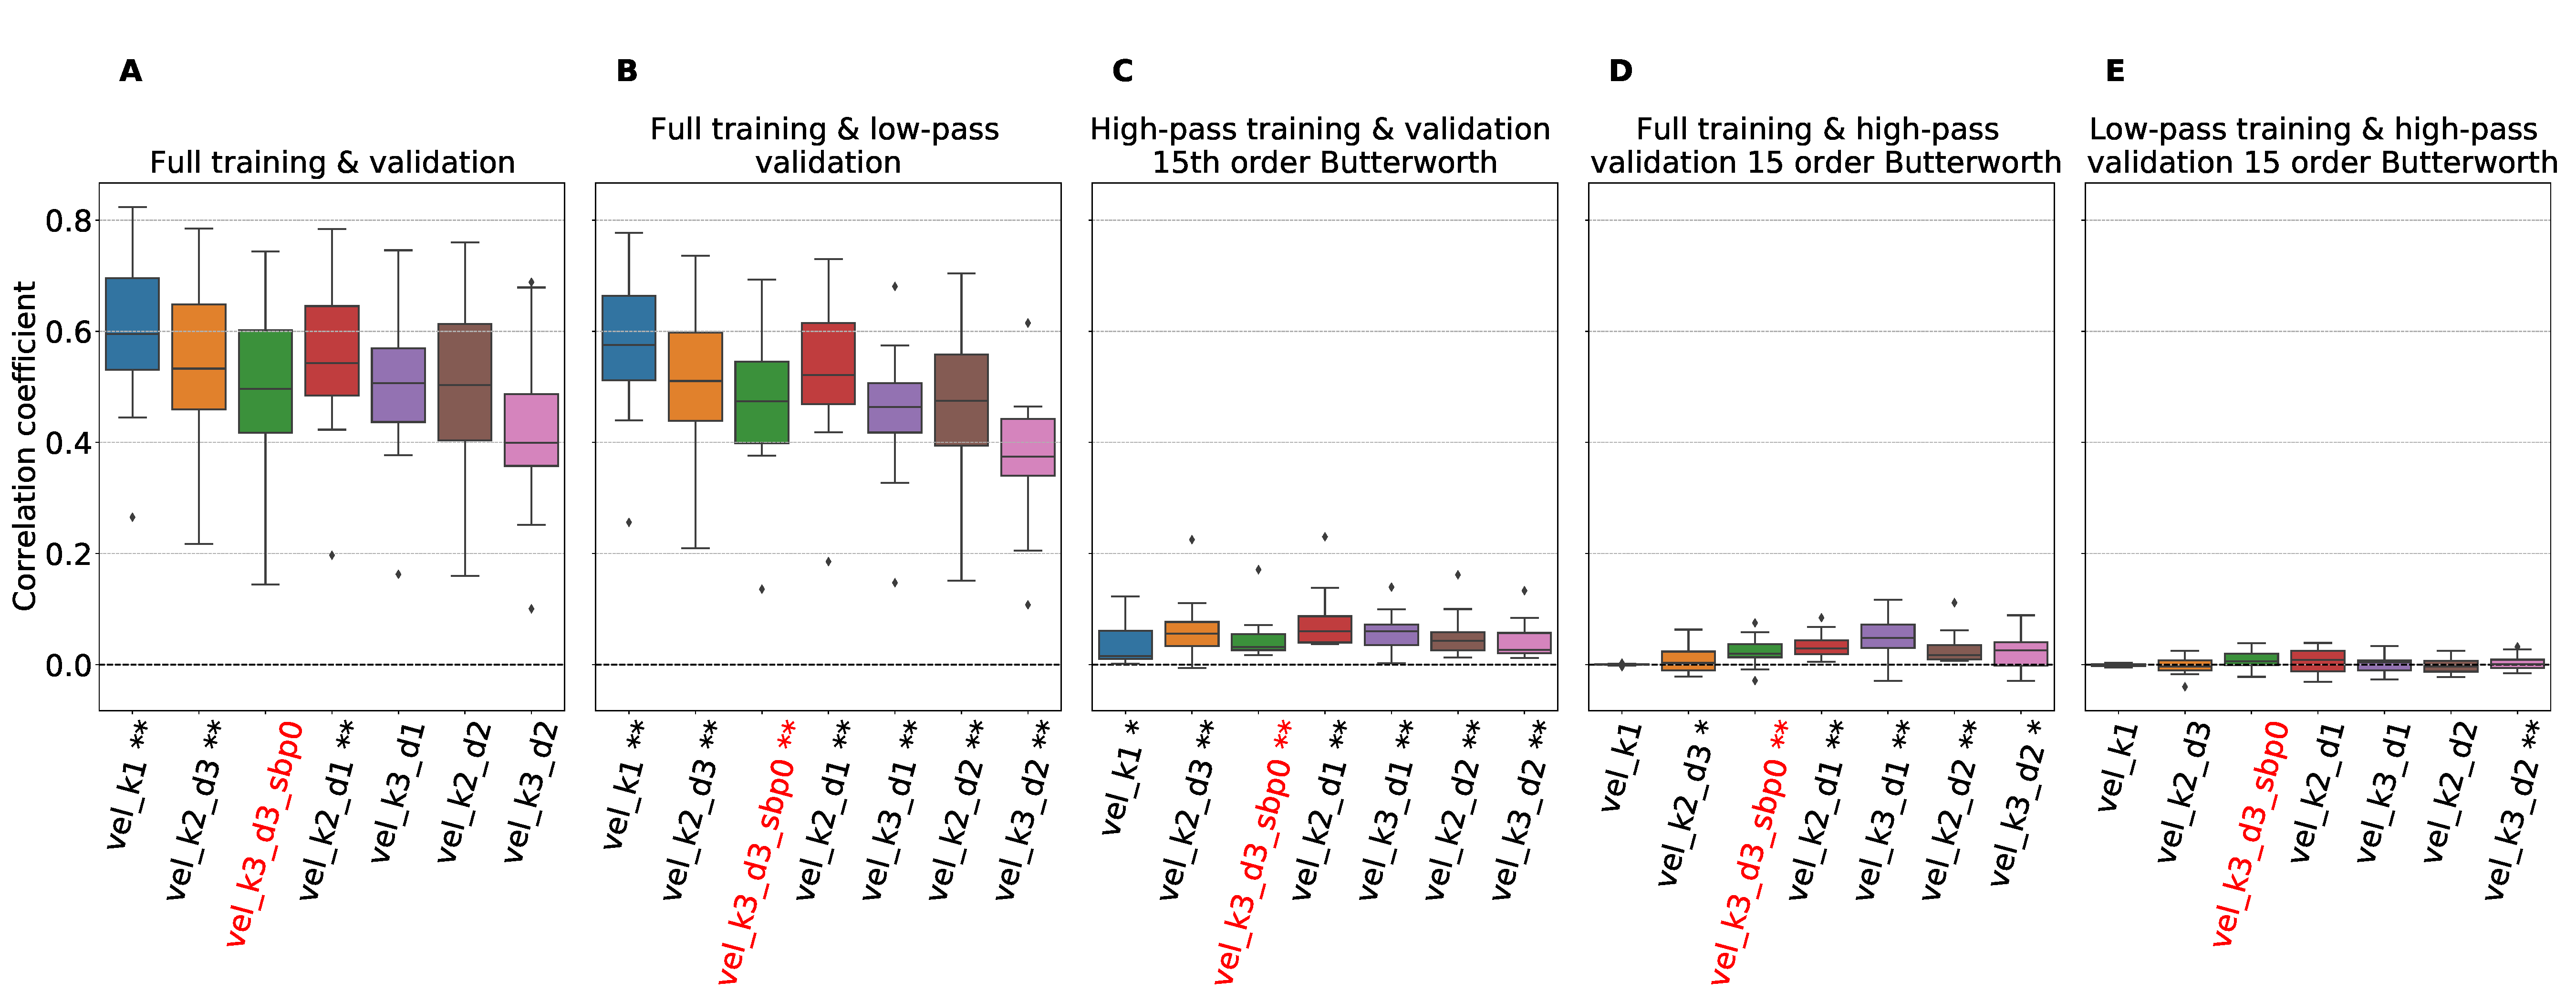
\includegraphics[width=1\linewidth]{img/ch4/original_setting_vel_performance_comparison}
   \caption{\textbf{Velocity} decoding correlation coefficients of the different CNNs established by architecture modifications. In all settings \textbf{
   A - E} the Deep4Net (vel\_k3\_d3\_sbp0) from~\cite{Hammer-2021} is labeled red. \textbf{Graph A} shows the performance of the networks when trained and validated on the full dataset. The stars in this case denote performance significantly above the vel\_k3\_d3\_sbp0. (** p <0.01), (* p < 0.05), Wilcoxon signed rank test.
   \textbf{Graph B} shows the correlation coefficients of the networks trained on full data and validated on low-passed data. 
   The stars denote if the drop of performance was significant between this setting and setting \textbf{A}. (** p <0.01), (* p < 0.05), Wilcoxon signed rank test.
   \textbf{Graph C} shows the performance of the CNNs when trained and validated on high-passed data. \textbf{Graph D} shows performance when trained on full data and validated on high-passed data. \textbf{Graph E} shows performance when trained on low-passed data and validated on high-passed data. For \textbf{Graphs C - E} the stars denote above chance performance - (** : p <0.01), (* : p < 0.05), Wilcoxon signed rank test.}
   \label{fig:original-performances-velocity} 
\end{subfigure}
\end{figure}

\begin{figure}
\ContinuedFloat

\begin{subfigure}[b]{\textwidth}
   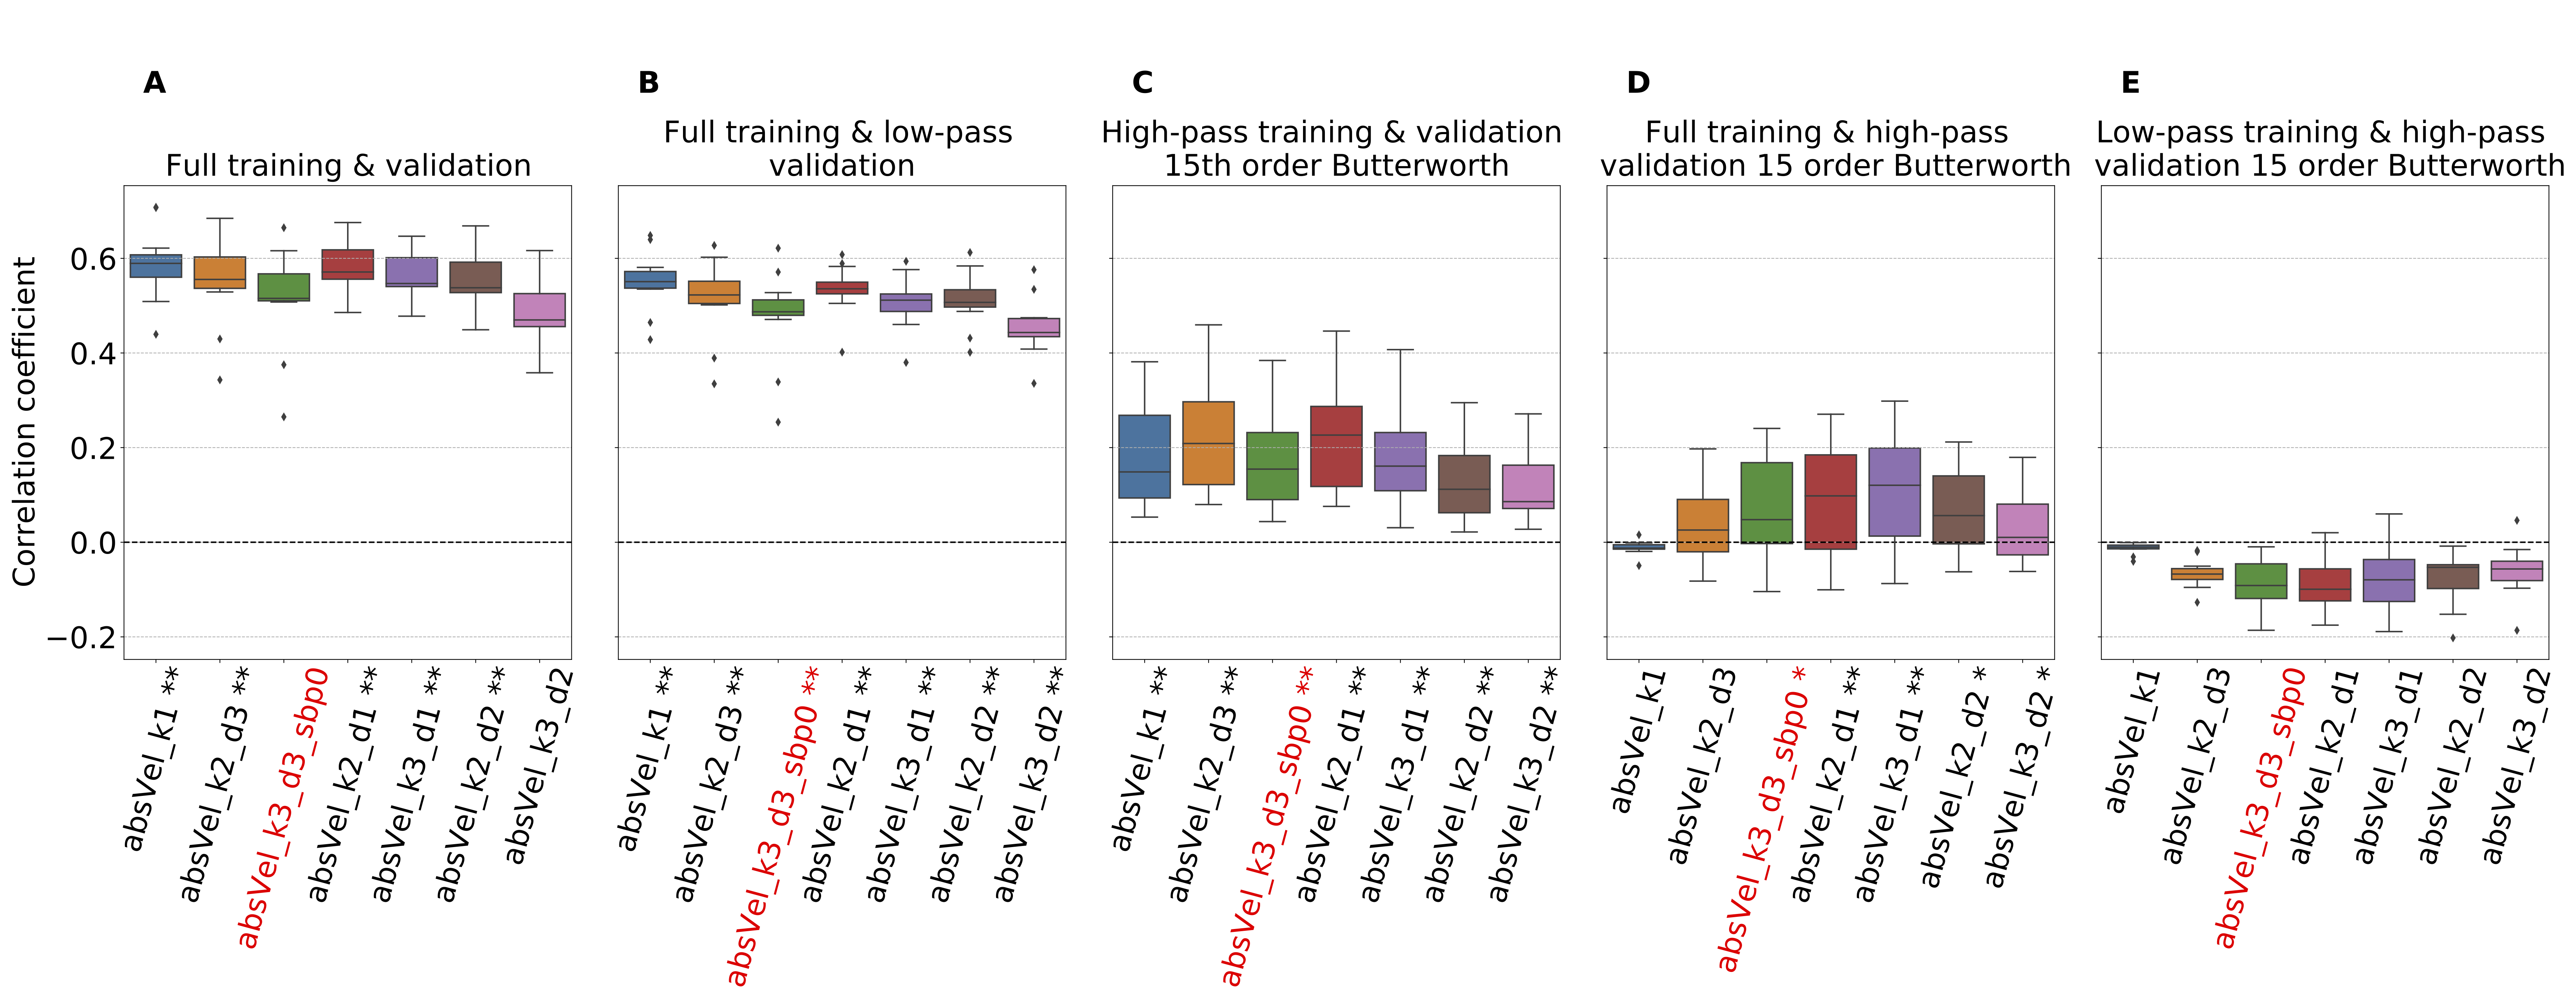
\includegraphics[width=1\linewidth]{img/ch4/original_setting_absVel_performance_comparison}
   \caption{\textbf{Absolute velocity} decoding correlation coefficients of the different CNNs established by architecture modifications. In all settings \textbf{
   A - E} the Deep4Net (absVel\_k3\_d3\_sbp0) from~\cite{Hammer-2021} is labeled red. \textbf{Graph A} shows the performance of the networks when trained and validated on the full dataset. The stars in this case denote performance significantly above the absVel\_k3\_d3\_sbp0. (** p <0.01), (* p < 0.05), Wilcoxon signed rank test.
   \textbf{Graph B} shows the correlation coefficients of the networks trained on full data and validated on low-passed data. 
   The stars denote if the drop of performance was significant between this setting and setting \textbf{A}. (** p <0.01), (* p < 0.05), Wilcoxon signed rank test.
   \textbf{Graph C} shows the performance of the CNNs when trained and validated on high-passed data. \textbf{Graph D} shows performance when trained on full data and validated on high-passed data. \textbf{Graph E} shows performance when trained on low-passed data and validated on high-passed data. For \textbf{Graphs C - E} the stars denote above chance performance - (** : p <0.01), (* : p < 0.05), Wilcoxon signed rank test.}
   \label{fig:original-performances-absolute-velocity}
\end{subfigure}
\caption[Non-shifted causal prediction - performances ]{}
\label{fig:original-performances}
\end{figure}


\end{itemize}

The findings presented in this section lead to two interesting questions.
The first one  is what do the gradients of the various architectures look like and do some of them use high-gamma?
This analysis is described in Section~\ref{subsec:gradients}.
The second question arises when we notice that the performance seems to drop with an increasing size of the receptive field: Figure~\ref{fig:figure-distance}.
Networks with a smaller receptive field seem to perform better possibly because the predicted time-point is closer to the centre of the receptive field. As described in more detail in Section~\ref{subsec:receptive-field} the non-uniformity of the receptive field together with causal prediction place the predicted time-point at the end of the receptive field while the network mostly focuses on the centre of the receptive field.
Therefore, it is interesting to see what happens when we shift the predicted time-point to the centre of the receptive field.
This analysis are described in Section~\ref{sec:shifting-the-predicted-time-point}.

\begin{figure}[!htpb]
\centering
\begin{subfigure}[b]{0.48\textwidth}
   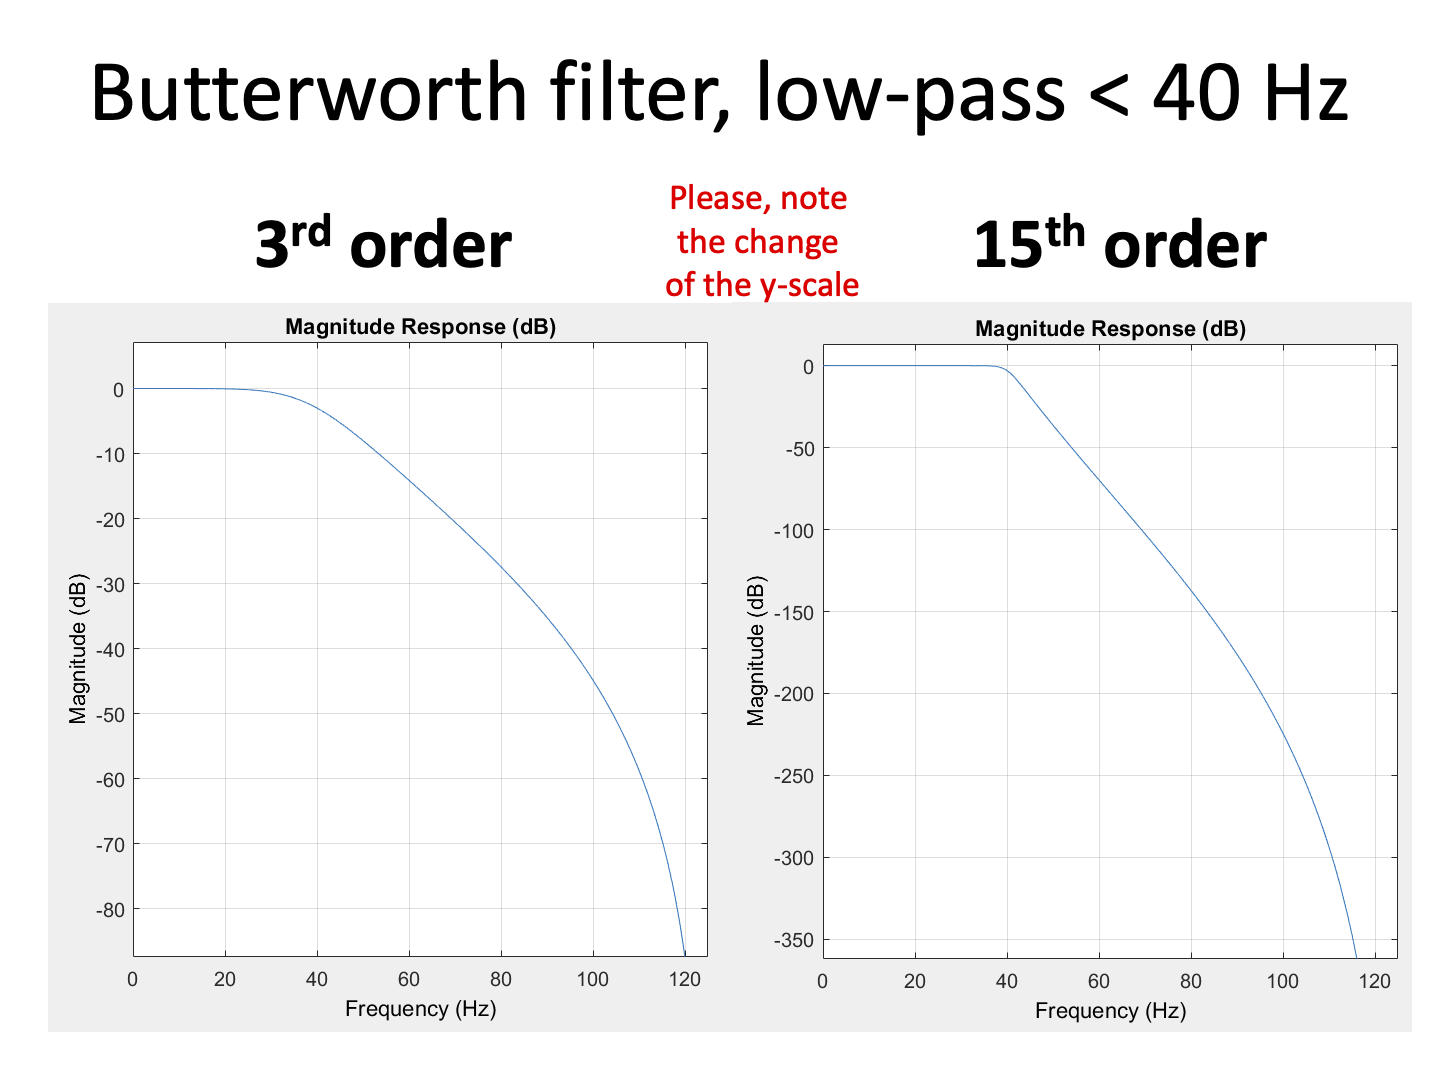
\includegraphics[width=1\linewidth]{img/ch3/lp-butterworth-filter}
   \caption{Comparison between 3rd and 15th order low-pass Butterworth filter, cutoff frequency 40~Hz}
   \label{fig:lp-filters}
\end{subfigure}
\begin{subfigure}[b]{0.48\textwidth}
   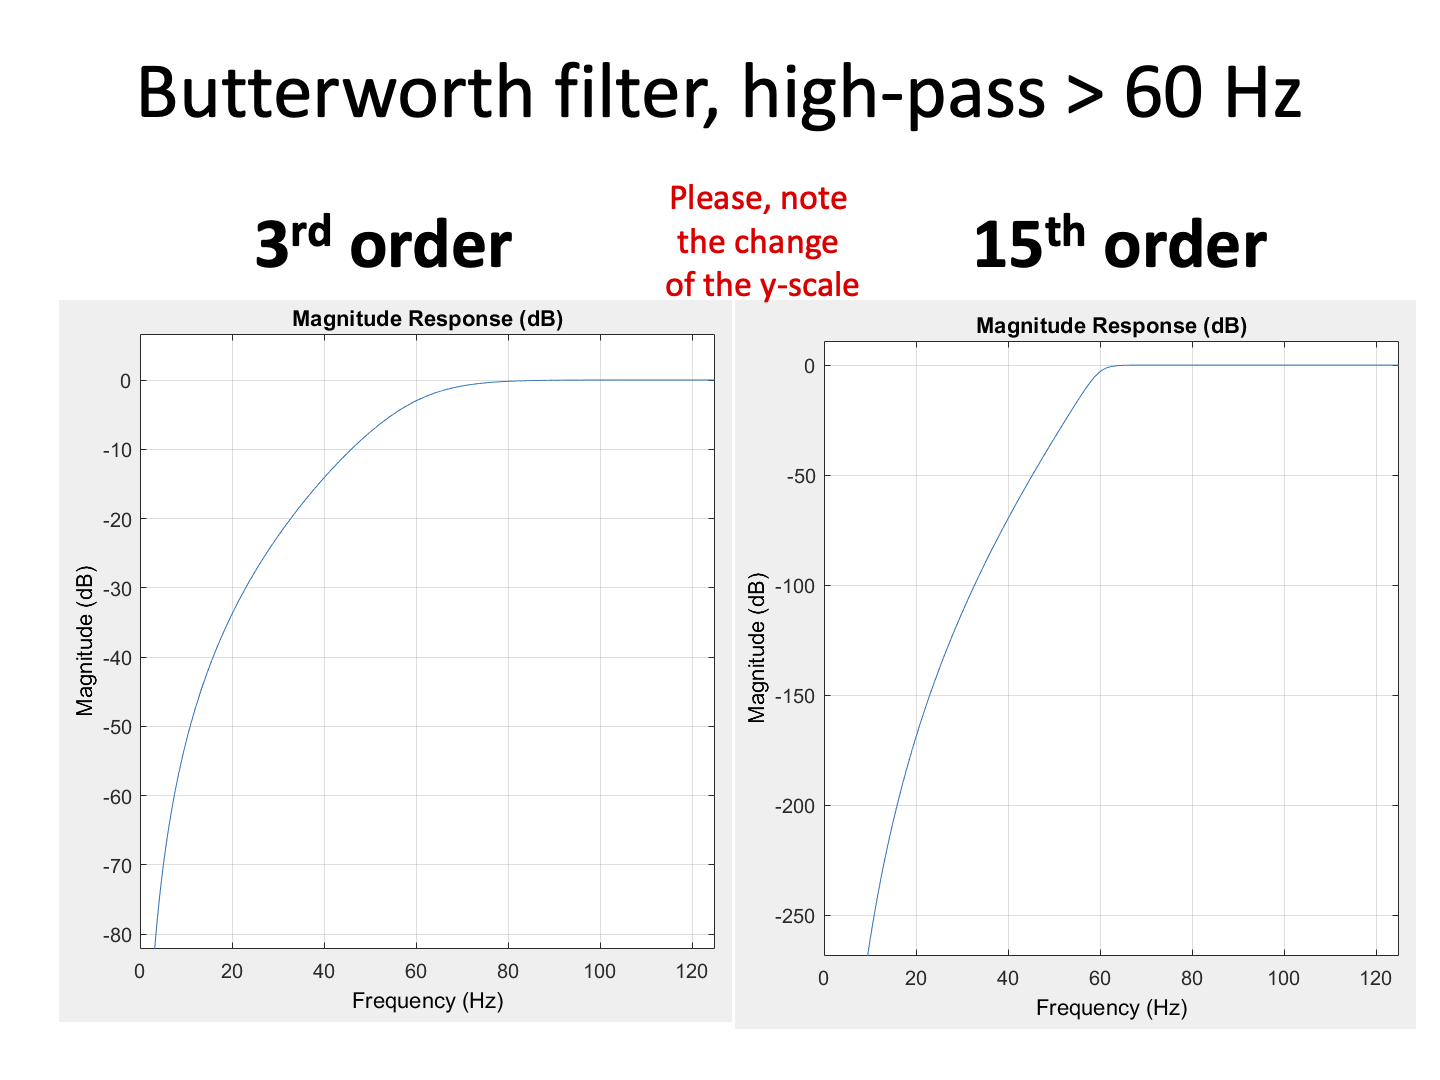
\includegraphics[width=1\linewidth]{img/ch3/hp-butterworth-filter}
   \caption{Comparison between 3rd and 15th order high-pass Butterworth filter, cutoff frequency 60~Hz}
   \label{fig:hp-filters}
\end{subfigure}
\caption[Butterworth filters - order comparison]{}
\label{fig:filters}
\end{figure}

\subsection{Gradients}\label{subsec:gradients}
The differences in performance among the networks, reinforce the interest in the gradients of the various architectures.
Since some of the networks perform significantly better compared to the initial Deep4Net, we analyze gradients of the different architectures to see if the reason for a better performance is their ability to use information from the high-gamma band.
We perform the gradient visualization of all the architectures with max-pool kernel sizes 1, 2 and 3 and dilations as powers of 1, 2 and 3.

The results show differences in gradients among the architectures.
Gradients of all intermediate layers and the visualizations can be found in Appendix~\ref{appendixA}.
Figure~\ref{fig:last-layer-grads} depicts the gradients of the output layer of each of the inspected architectures. The output layer in our opinion best represents the gradients of the other layers.

\begin{figure}[!htpb]
\centering
\begin{subfigure}[b]{\textwidth}
   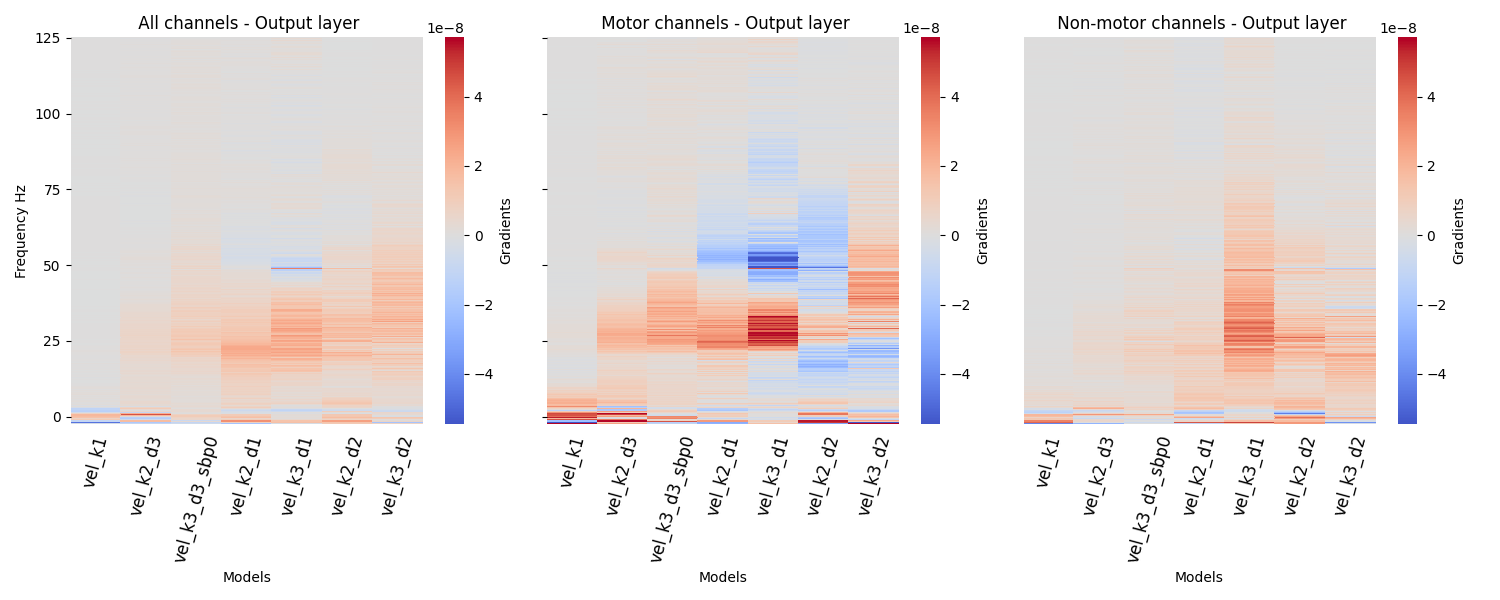
\includegraphics[width=1\linewidth]{img/ch4/vel-last-layer-grads}
   \caption{}
   \label{fig:absVel-last-layer-grads}
\end{subfigure}

\begin{subfigure}[b]{\textwidth}
   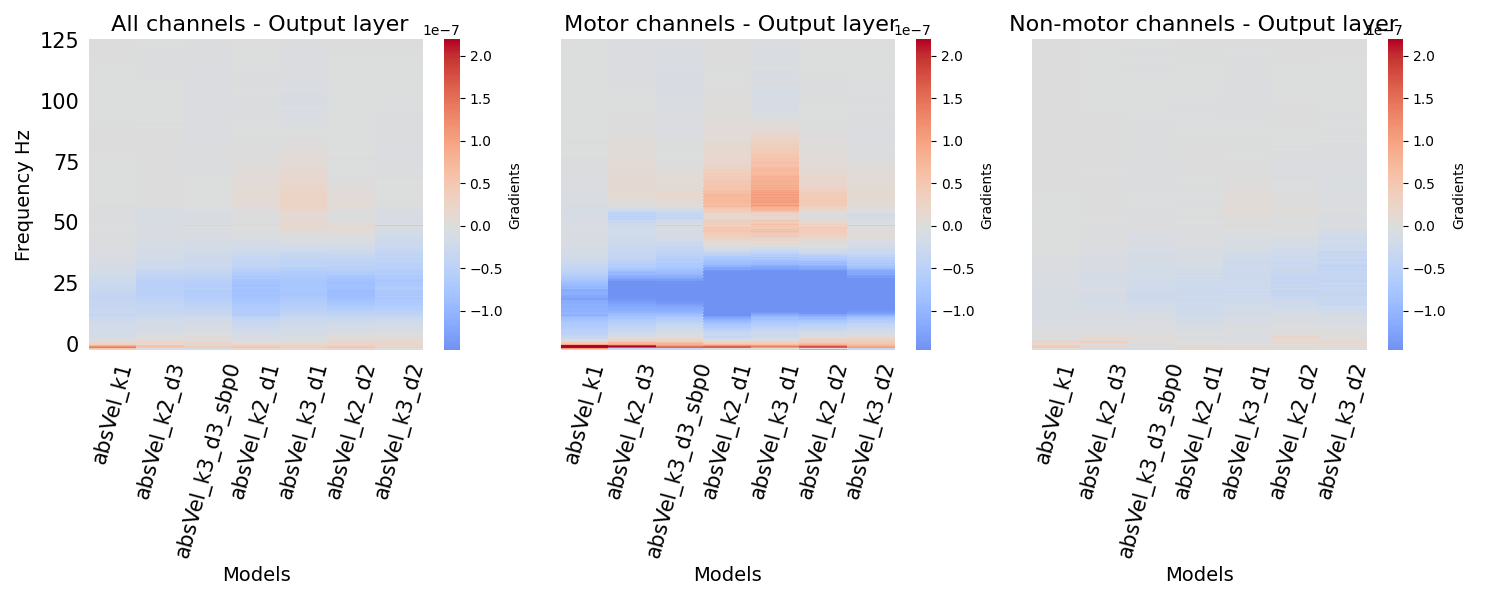
\includegraphics[width=1\linewidth]{img/ch4/absVel-last-layer-grads}
   \caption{}
   \label{fig:vel-last-layer-grads}
\end{subfigure}
\caption[Non-shifted causal prediction - gradients]{Gradients of the different CNN architectures decoding \textbf{(a) Velocity} and \textbf{(b) Absolute velocity}. All channels include channels that do not belong to motor neither non-motor channel sets. See Section \ref{subsec:ieeg-data-preprocessing}}
\label{fig:last-layer-grads}
\end{figure}

Based on the performances of the networks presented in Section~\ref{subsec:performance} and the gradients presented in this Section these important and interesting observations can be made:

\begin{itemize}
    \item The networks focus mostly on motor-channels when making predictions.
This is to be expected when they are tasked with decoding movement.
    \item There are obvious differences between the gradients for velocity and absolute velocity.
    Nevertheless, networks with interest in wider frequency ranges for velocity decoding have interest in wider frequency ranges for absolute velocity decoding and vice-versa.
    \item For both variables the network without max-pool, denoted as \{variable\}\_k1 is the best performing architecture.
    And in both cases is it also the network which is most interested in modulations in the low frequency bands.
    This suggests that using the information in the high-gamma frequency band is not necessarily an asset.
    \item The networks which exhibit higher interest in information from the higher frequencies, namely the \{variable\}\_k2\_d1, \{variable\}\_k3\_d1 and \{variable\}\_k2\_d2 are also those, which are able to perform significantly above chance when trained on full data and validated on high-passed data for both velocity and absolute velocity.
    This suggests consistency between the gradient visualization and the performance analysis.

\end{itemize}


\section{Shifting the predicted time-point}\label{sec:shifting-the-predicted-time-point}
In this section we describe how the performance and gradients change when the predicted time-point is shifted with respect to the receptive field. In Section~\ref{subsec:receptive-field} we described how the non-uniformity of the receptive field causes the network to focus on information from the centre of its receptive field while the predicted time-point lies at the edge of the receptive field to allow for causal prediction. To see what happens if we shift the predicted time-point across the receptive field\footnote{By shifting the predicted time-point from the edge of the receptive field we are giving up causal prediction.} two kinds of analyses are introduced here.

\begin{enumerate}
    \item Shifting the predicted time-point to the centre of the receptive field.
This analysis was performed on all the network architectures and compares how the different architectures react to the shift, both performance-wise and gradient-wise.
We highlight the differences and similarities between the architectures.
    \item Shifting the predicted time-point in steps across the receptive field.
This analysis was performed only on the original Deep4Net which we denote as \{variable\}\_k3\_d3\_sbp0.
It compares how the performance and gradients of the network change when the predicted time-point is shifted across the receptive field, using a different ratio of information from the future and from the past.
\end{enumerate}


\subsection{Shifting the predicted time-point to the centre of the receptive field}\label{subsec:shifting-the-predicted-time-point-to-the-centre-of-the-receptive-field}
An important observation when looking at the performance of the different architectures described in Section~\ref{sec:architectural-modifications} was made.
We noticed that a smaller receptive field seemingly correlates with a higher prediction accuracy especially for absolute velocity decoding.
To visualize this, we created Figure~\ref{fig:figure-distance} which sorts the different architectures based on the size of the receptive field from smallest to largest and plots the average correlation coefficient each of these networks achieved.
There is a clear descending pattern especially for absolute velocity where the only exceptional network is the k3\_d3 network which performs well with a relatively large receptive field.


\begin{figure}[!htbp]
\centering
   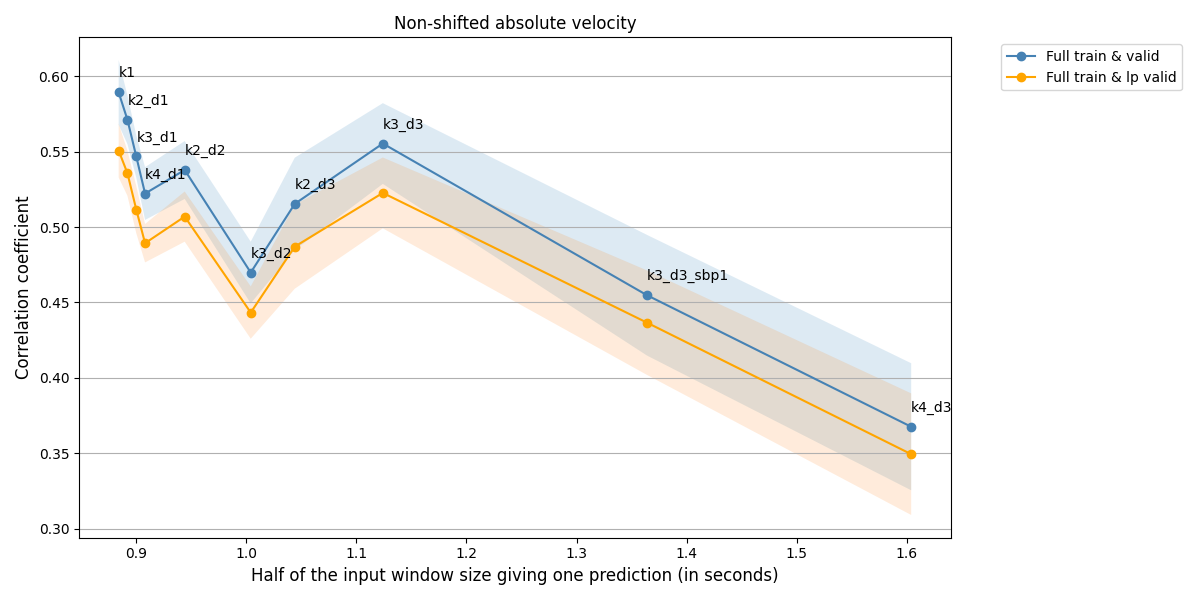
\includegraphics[width=1\linewidth]{img/ch4/distance-shifted-performance-absVel}
   \caption[Dependence of performance on receptive field size]{The average performance of the different CNN architectures with respect to the size of their receptive field. Blue: Full training and validation CC; Light-blue: full training and validation CC standard deviation; Orange: Full training and low-pass validation CC; Light-orange: Full training and low-pass validation CC standard deviation}
   \label{fig:figure-distance}
\end{figure}

We described in Section~\ref{subsec:receptive-field} that the receptive field is non-uniform - it considers mostly input-points in its centre; and that in the original, non-shifted setting (causal prediction), the predicted time-point is located just outside the receptive field which places it relatively far from the centre of the receptive field. 
This and the descending pattern of the performance with an increasing receptive field size from Figure~\ref{fig:figure-distance}, corroborate the hypothesis that the distance of the predicted time-point to the centre of the receptive field plays an important role in the prediction power of the architectures.
Smaller size of the receptive field means smaller distance between predicted time-point and receptive field centre and therefore, possibly access to more relevant signals recorded closer to the predicted movement execution.

To study this further, we shift the inputs and predictions so that the iEEG signal, which was recorded at the same time as the predicted movement was executed, is in the centre of the receptive field\footnote{This causes the procedure to be unsuitable for online BCI because half of the input window uses information from the future.}. 
We present how this affects the performances and gradients of the various architectures.

\subsubsection{Performance}
The performance related results are displayed in Figure~\ref{fig:shifted-performance}.
We summarize how the shift influences performances on the different datasets in the following points:
\begin{itemize}
    \item \textbf{Full training and validation:} It is obvious that the shift greatly improves performance of all the networks on the original full data training and validation and that in this setting the performance differences between the architectures are diminished.
    
    
    \item \textbf{Full training and low-pass validation} After the shift, the performance of the networks in the shifted setting drops significantly for all the networks as it does in the non-shifted original setting. This suggests that the networks use some information from frequencies above 40~Hz in the shifted setting.
    
    \item \textbf{High-pass training and validation} The performance of the networks on the high-gamma dataset increases with the shift, especially for absolute velocity. This suggests that the modulations in the frequencies above 60~Hz become more informative with the shift.
    
    \item \textbf{Full training and high-pass validation} After the shift, the performance of the networks trained on full data and validated on high-pass data decreased. For absolute velocity and velocity, less networks were able to perform above chance level and those which stayed above chance level often perform above chance level less significantly. This suggests that the networks, when having access to full data, depend on the information from the high frequencies less than in the original non-shifted setting.

\end{itemize}


\begin{figure}[!htpb]
\centering
\begin{subfigure}[t]{\textwidth}
   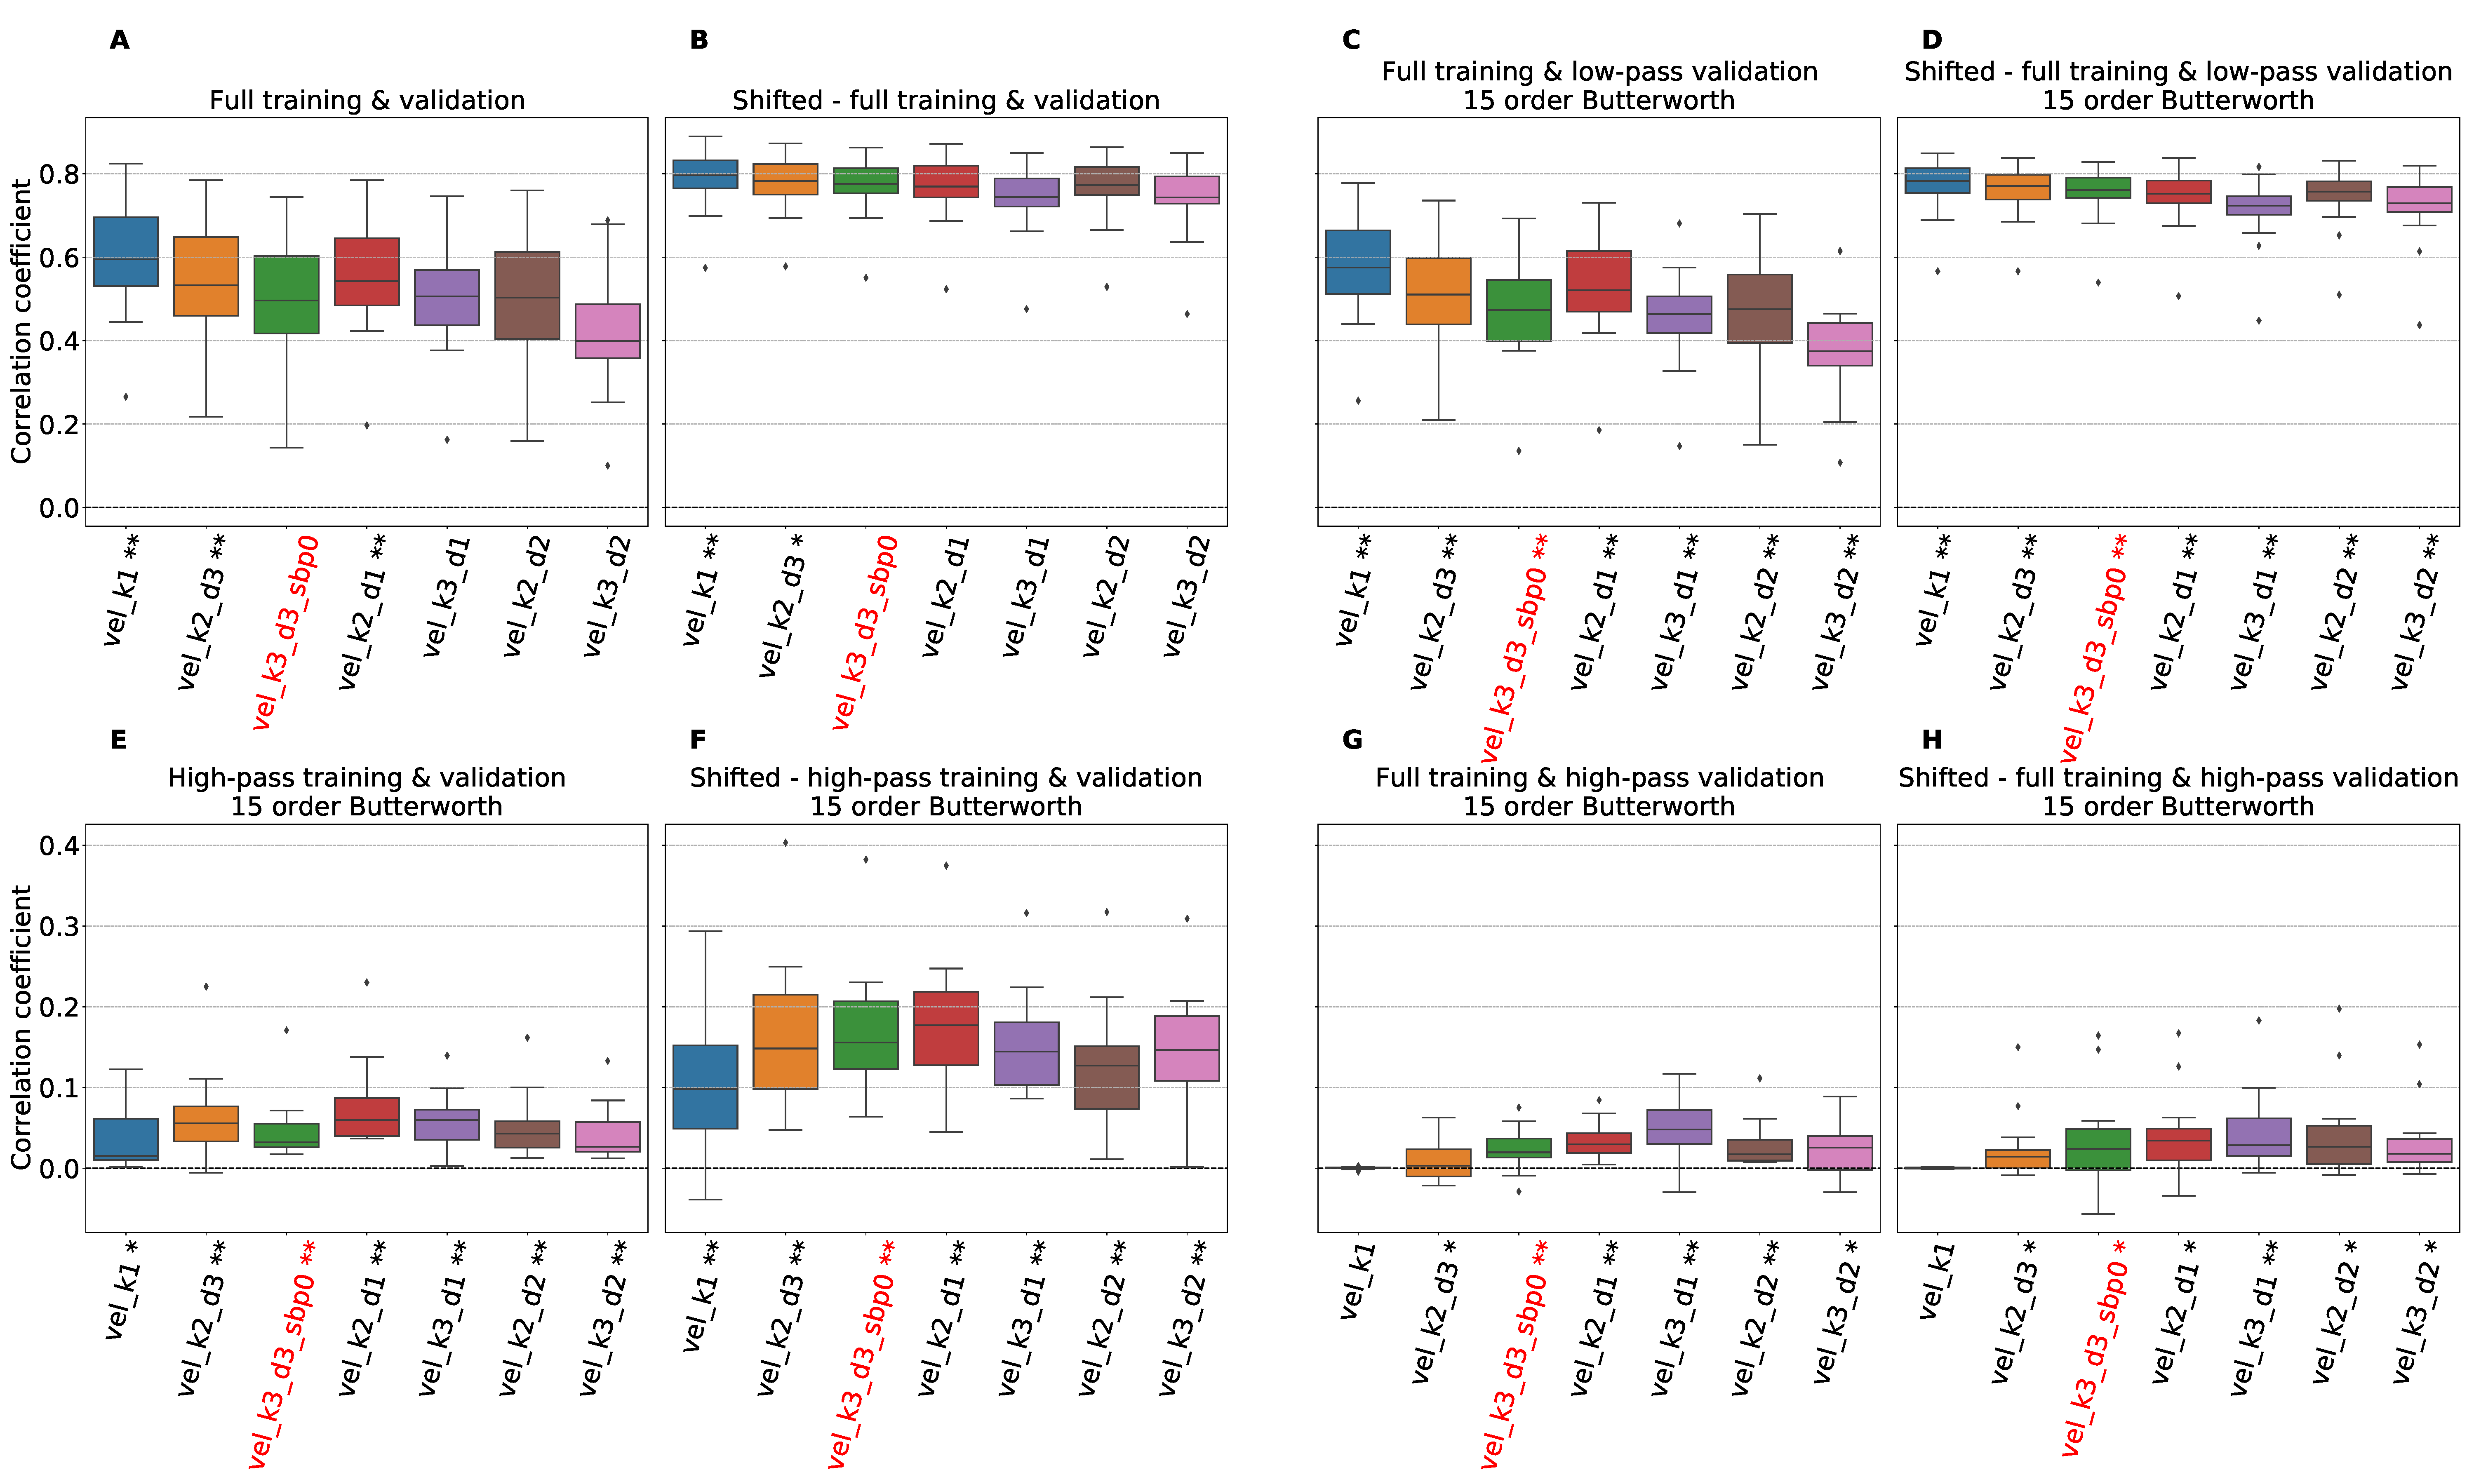
\includegraphics[width=1\linewidth]{img/ch4/original_vs_shifted_vel_performance_comparison.pdf}
   \caption[Velocity: non-shifted vs. shifted setting performances]{\textbf{Velocity} decoding correlation coefficients comparison between original causal prediction \textbf{Graphs A, C, E, G} and the shifted (acausal) prediction \textbf{Graphs B, D, F, H}. In all settings \textbf{
   A - E} the Deep4Net (k3\_d3\_sbp0) from~\cite{Hammer-2021} is labeled red.\\ \textbf{Graphs A} and \textbf{B} compare the performance of the networks when trained and validated on the full dataset. A The stars in \textbf{A} and \textbf{B} denote performance significantly above the Deep4Net in the same setting. (** p <0.01), (* p < 0.05), Wilcoxon signed rank test.
   \\\textbf{Graphs C} and \textbf{D} show the correlation coefficients of the networks trained on full data and validated on low-passed data. 
   The stars in \textbf{C} denote if the CCs are significantly lower compared to \textbf{A}. The stars in \textbf{D} denote if the CCs are significantly lower compared to \textbf{B}. (** p <0.01), (* p < 0.05), Wilcoxon signed rank test.
   \\\textbf{Graphs E} and \textbf{F} compare the CCs of the CNNs when trained and validated on high-passed data. \textbf{Graphs G} and \textbf{H} compare performance when trained on full data and validated on high-passed data. For \textbf{Graphs E - H} the stars denote above chance performance - (** : p <0.01), (* : p < 0.05), Wilcoxon signed rank test.}
   \label{fig:shifted-performance-vel}
\end{subfigure}
\end{figure}
\clearpage   

\begin{figure}[!htbp]\ContinuedFloat
\begin{subfigure}[t]{\textwidth}
   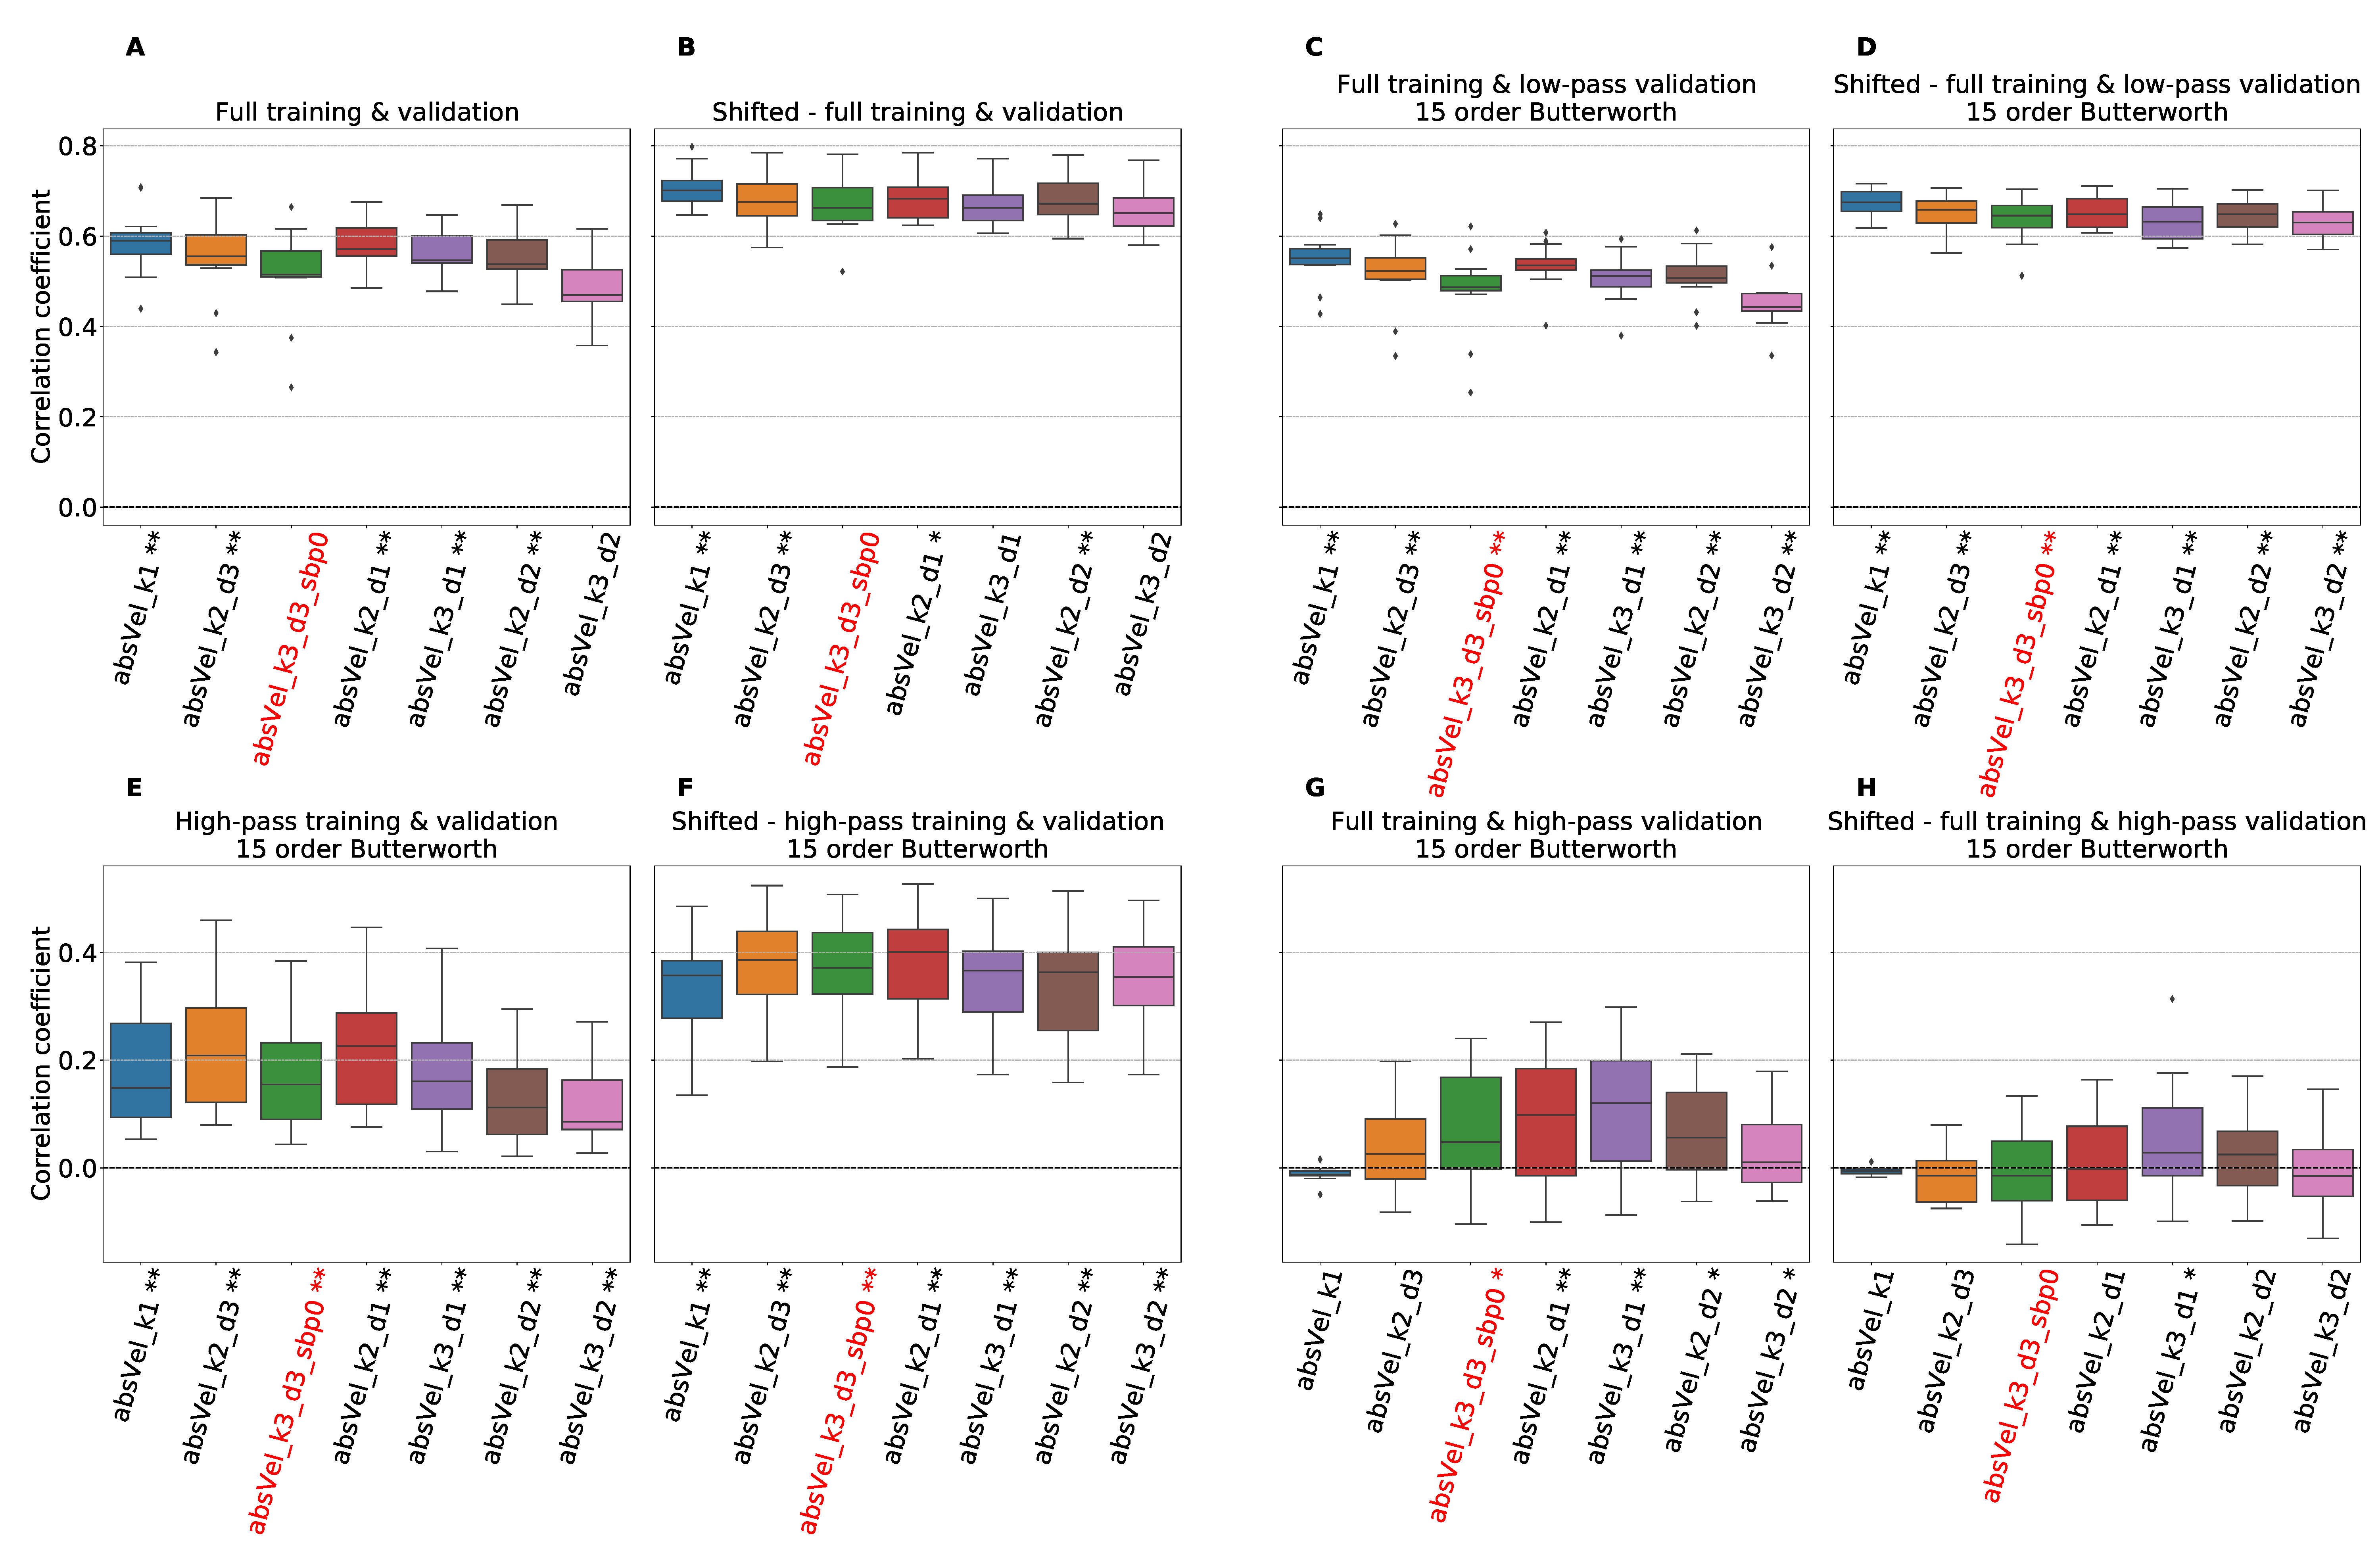
\includegraphics[width=1\linewidth]{img/ch4/original_vs_shifted_absVel_performance_comparison.pdf}
   \caption{}
   \label{fig:shifted-performance-absVel}
\end{subfigure}
\caption[Absolute velocity: non-shifted vs. shifted setting performances]{{\textbf{Absolute velocity} decoding correlation coefficients comparison between original causal prediction \textbf{Graphs A, C, E, G} and the shifted (acausal) prediction \textbf{Graphs B, D, F, H}. In all settings \textbf{
   A - E} the Deep4Net (k3\_d3\_sbp0) from~\cite{Hammer-2021} is labeled red.\\ \textbf{Graphs A} and \textbf{B} compare the performance of the networks when trained and validated on the full dataset. A The stars in \textbf{A} and \textbf{B} denote performance significantly above the Deep4Net in the same setting. (** p <0.01), (* p < 0.05), Wilcoxon signed rank test.
   \\\textbf{Graphs C} and \textbf{D} show the correlation coefficients of the networks trained on full data and validated on low-passed data. 
   The stars in \textbf{C} denote if the CCs are significantly lower compared to \textbf{A}. The stars in \textbf{D} denote if the CCs are significantly lower compared to \textbf{B}. (** p <0.01), (* p < 0.05), Wilcoxon signed rank test.
   \\\textbf{Graphs E} and \textbf{F} compare the CCs of the CNNs when trained and validated on high-passed data. \textbf{Graphs G} and \textbf{H} compare performance when trained on full data and validated on high-passed data. For \textbf{Graphs E - H} the stars denote above chance performance - (** : p <0.01), (* : p < 0.05), Wilcoxon signed rank test.}}
   \label{fig:shifted-performance}
\end{figure}
\clearpage
The overall improvement in performance can be caused by two things:
\begin{enumerate}
    \item By the network being able to focus on signals recorded directly before the movement execution.
    \item By the network having access to information from the future.
\end{enumerate}

We hypothesise that is most likely a combination of the two.
Conclusion about how much each of the above described possibilities influences the prediction improvement cannot be made from the presented experiments.
It would be interesting to build a network with a uniform receptive field and then conduct experiments which would clarify this.

If the performance improvement was caused solely or mainly by access to information directly preceding the predicted time-step a network with a uniform receptive field (one which allows padding) could potentially bring an improvement, similar to the one we achieved by shifting the predicted time-point, while retaining its usability for online BCI.
Nevertheless, such an analysis is out of the scope of this thesis.

On a side note, we can see in Figures \ref{fig:shifted-performance-vel} and \ref{fig:shifted-performance-absVel} that when training and validating on the full data in shifted setting (Graphs B) the velocity correlation coefficients are higher than the absolute velocity correlation coefficients. 
This seems a bit counter-intuitive because absolute velocity can be derived from velocity only using the absolute value of velocity. 
Therefore, it could be at least as well decoded.
To see if indeed absolute velocity can be decoded better when taking absolute values of velocity we trained a network on velocity data and validated it on absolute values of the predictions and absolute velocity data.
The results show that the correlation coefficients are significantly worse than when training the network on absolute velocity data (Figure~\ref{fig:absVel-vs-abs-vel-performance}). Even though it seems that it might be better to learn to decode absolute velocity as velocity and then take the absolute value, we find that it is not. 

This might come as surprising but can be explained mathematically. The correlation coefficient is derived from the mean and standard deviation of the variables as:

\begin{equation}
    CC_{(X, Y)}= \frac{E[(X - \mu_X)(Y - \mu_Y)] }{\sigma_x \sigma_y}
    \label{eq:correlation}
\end{equation}

where $X$ and $Y$ are two random variables $\sigma_x, \sigma_y$ are the standard deviations of X and Y, $ \mu_x, \mu_y$ are the means of X and Y.

There is no equitation that would tell us how absolute value changes the mean and standard deviation of an arbitrary variable. Therefore, the means and standard deviations of the predicted values and the gold values change independently when taking their absolute values and the correlation coefficient changes.
It is not equivalent to take the correlation coefficients of two variables and the correlation of absolute values of two variables. 
To show this non-equivalency, let $X$ be a random variable with values $X = \{1, 0, 1, 0, 1\} $ and $Y$ be a random variable with values $Y = \{2, 1, -2, 1, 2\}$. In this case $CC_{(X,Y)} = -0.1111$ and $CC_{(|X|,|Y|)} = 1$.

    
\begin{figure}[!htpb]
\centering
   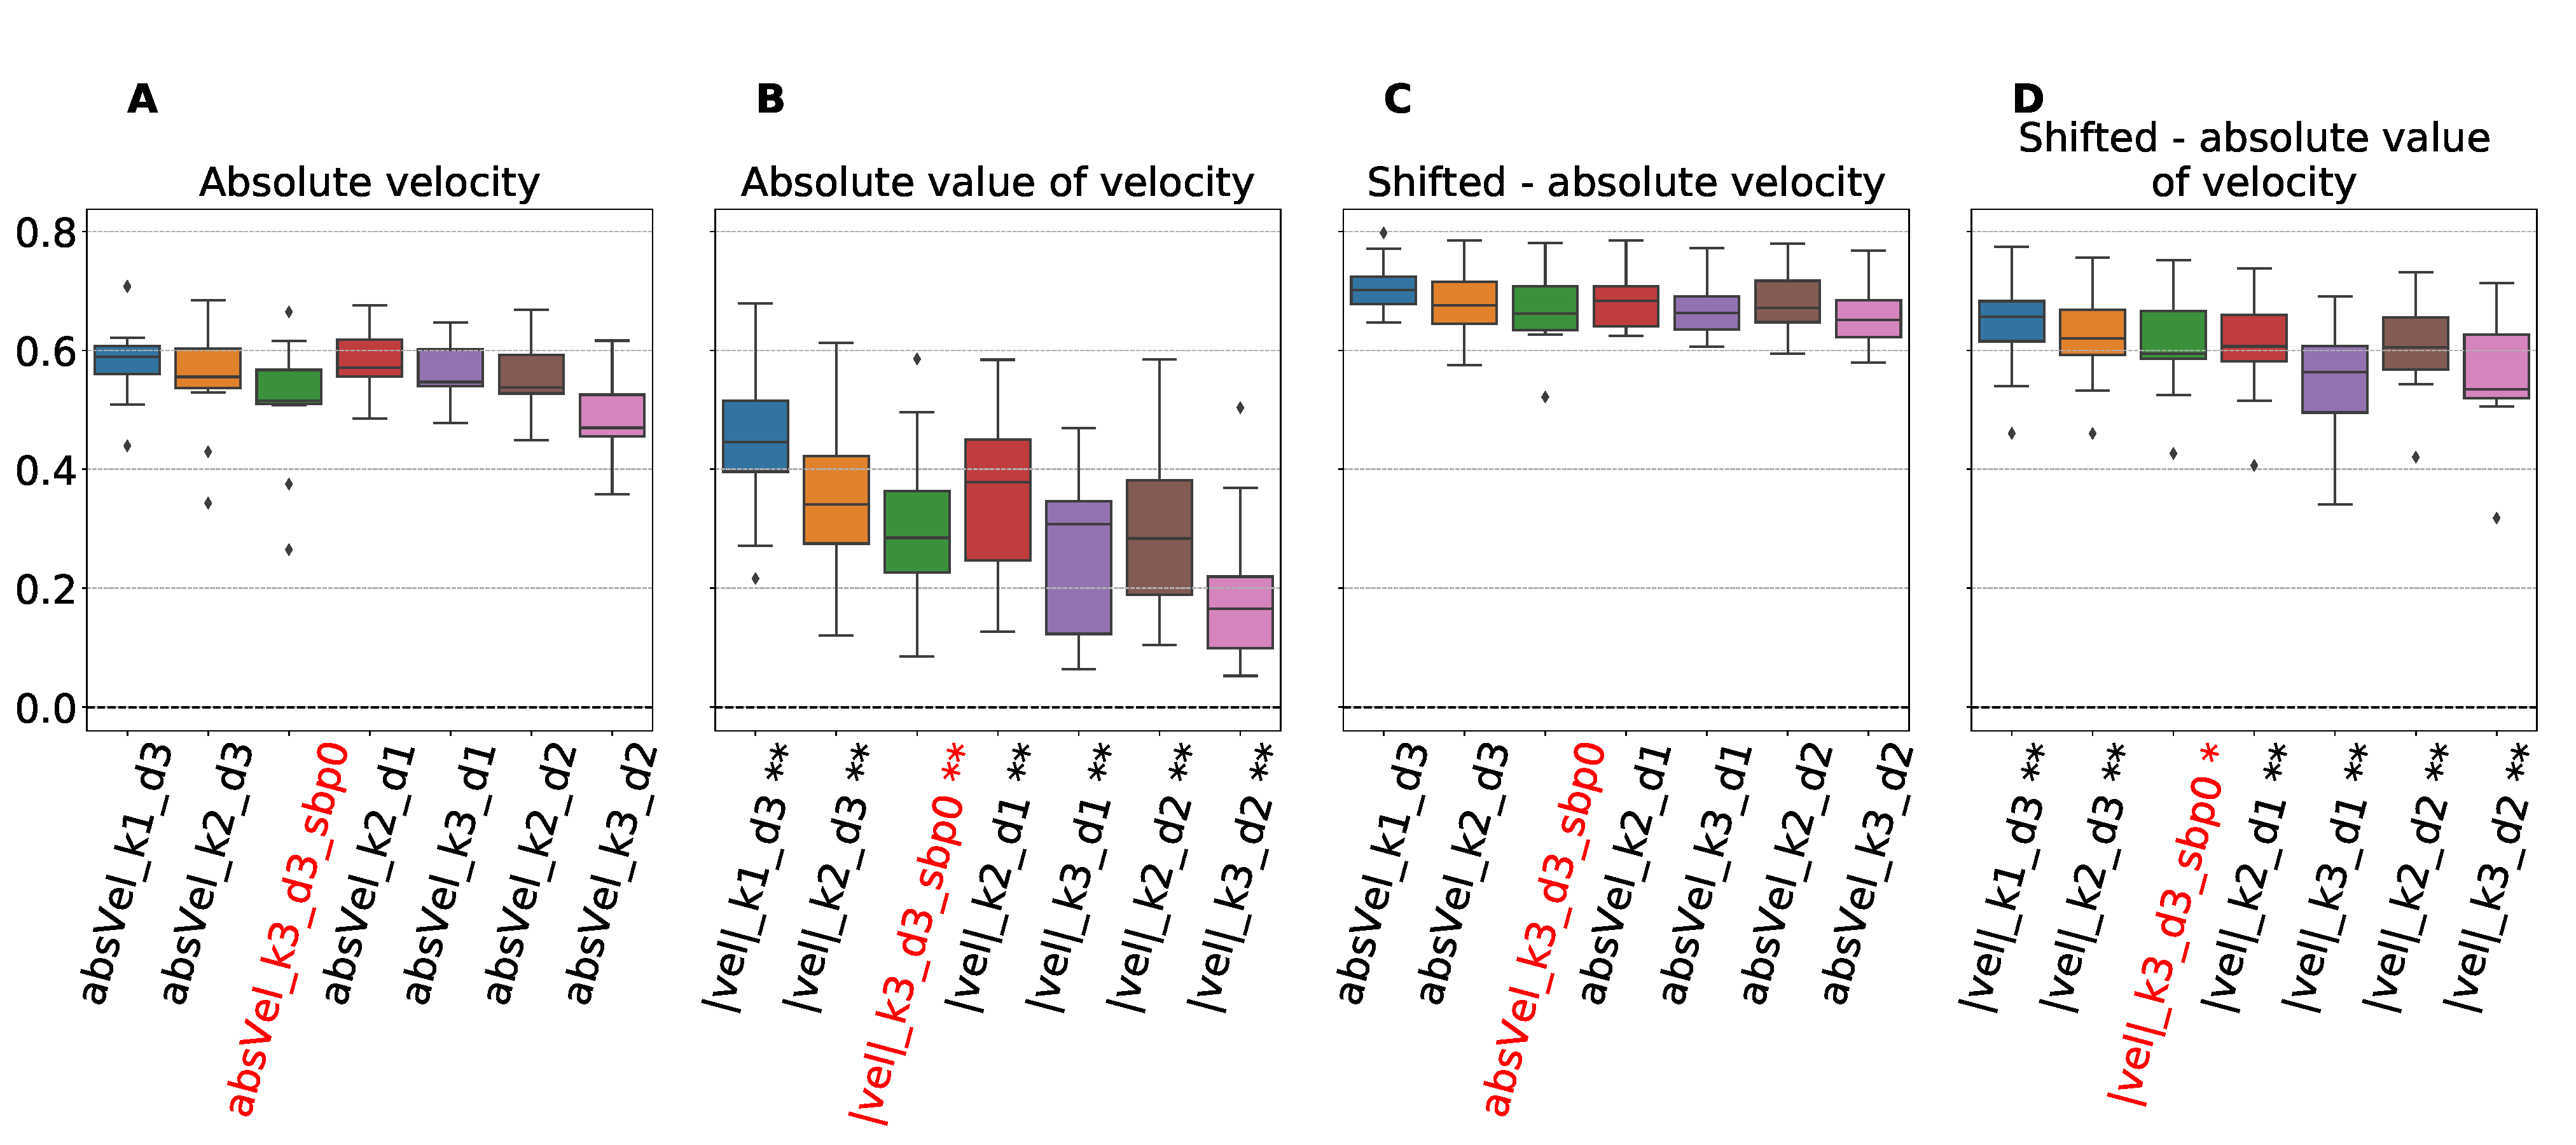
\includegraphics[width=1\linewidth]{img/ch4/absVel_vs_abs_vel_performance_comparison}
   \caption[Absolute velocity vs. absolute value of velocity comparison]{Absolute velocity decoding from a absolute velocity data \textbf{Graphs A, C} and absolute velocity decoding when taking absolute values of networks trained on velocity data \textbf{Graphs B, D}. In all settings \textbf{
   A - D} the Deep4Net (k3\_d3\_sbp0) from~\cite{Hammer-2021} is labeled red.\\ \textbf{Graphs A} and \textbf{B} compare the performance of the networks when trained and validated on the full dataset. A The stars in \textbf{B} denote performance significantly below the same architecture in graph \textbf{A}. (** p <0.01), (* p < 0.05), Wilcoxon signed rank test.
   \\\textbf{Graphs C} and \textbf{D} compare the performance of the networks when trained and validated on the full dataset in the shifted setting. A The stars in \textbf{D} denote performance significantly below the same architecture in graph \textbf{C}. (** p <0.01), (* p < 0.05), Wilcoxon signed rank test.}
   \label{fig:absVel-vs-abs-vel-performance}
\end{figure}


\subsubsection{Gradients}
We theorised that the information about the velocity and absolute velocity of the movement could be encoded in the high-gamma frequencies of iEEG only in the moments directly preceding the movement.
Therefore, the networks were unable to use it in the original non-shifted setting because they were biased towards signals recorded too far in the past (see Section \ref{subsec:receptive-field}).
The drop of performance of the networks after the shift when trained on full data and validated on high-passed data visible in Figure~\ref{fig:shifted-performance} speaks against this theory. 
To further test this hypothesis, we compared the gradients between the networks in the original non-shifted setting (causal prediction) and the shifted setting where the predicted time point is in the centre of the receptive field (acausal prediction).
This analysis was performed for all the architectures for all their intermediate convolutional layers\footnote{omitting the temporal and spatial convolution} on 1. the full dataset and 2. the high-passed dataset.
The complete results can be found in Appendix~\ref{appendixB}.
Below, we show results from the convolutional layer in the third convolutional block (conv\_3) which serves as representation of the overall trend. 

\begin{enumerate}
    \item Gradients of networks which are \textbf{trained and validated on full data} are displayed in Figures~\ref{fig:vel-shifted-vs-non-shifted-grads} (velocity) and~\ref{fig:absVel-shifted-vs-non-shifted-grads} (absolute velocity).
    What we observe is that with the shift the networks across all architecture seem to refine their focus to more narrow frequency bands.
    This can be illustrated on for example Figure~\ref{fig:vel-conv3-layer-grads} where in the original, non-shifted setting, the vel\_k1 network has high-gradient values for frequencies up to 25~Hz when looking at motor channels.
    In the shifted setting Figure~\ref{fig:vel-conv3-layer-grads-shifted} the band with high gradient values of the same network vel\_k1 narrows to frequencies closer to 0.
    
    For no network  did the shift cause an increase in the use of information from the high-gamma frequency band.
    Rather it seems, that the shift allowed access to less noisy information in the clearly informative bands such as the alpha and beta bands, and the network did not compensate with information from other frequencies.
    
    \item Networks which were \textbf{trained and validated on high-passed data} can be found in Figures~\ref{fig:vel-shifted-vs-non-shifted-grads-hp} (velocity) and~\ref{fig:absVel-shifted-vs-non-shifted-grads-hp} (absolute velocity).
    Again, we only chose to display gradients of one layer to illustrate a behaviour shared by all layers.
    The gradients of the remaining layers can be found in Appendix~\ref{appendixB}.
    What we observe in the gradients of the networks trained on high-passed datasets is different (even opposite) from what we observe in gradients of networks trained on the full dataset.
    The networks trained on high-passed data in the shifted setting exhibit interest in the same or a broader range of frequencies above the 60~Hz cut-off frequency than the networks trained on high-passed data in the original, non-shifted setting.
    This and the increase in performance on high-passed datasets suggests that indeed the information in high-frequency bands in signals from the future or directly preceding the movement contains more information about movement.
    But the fact that the networks trained in the shifted setting on full data do not increasingly use high-gamma, while their performance increases significantly compared to the non-shifted setting, points to the information in high-gamma being informative but redundant when having access to information from all frequencies.
\end{enumerate}

\begin{figure}[!htpb]
\centering
\RawFloats
\begin{subfigure}[b]{\textwidth}
   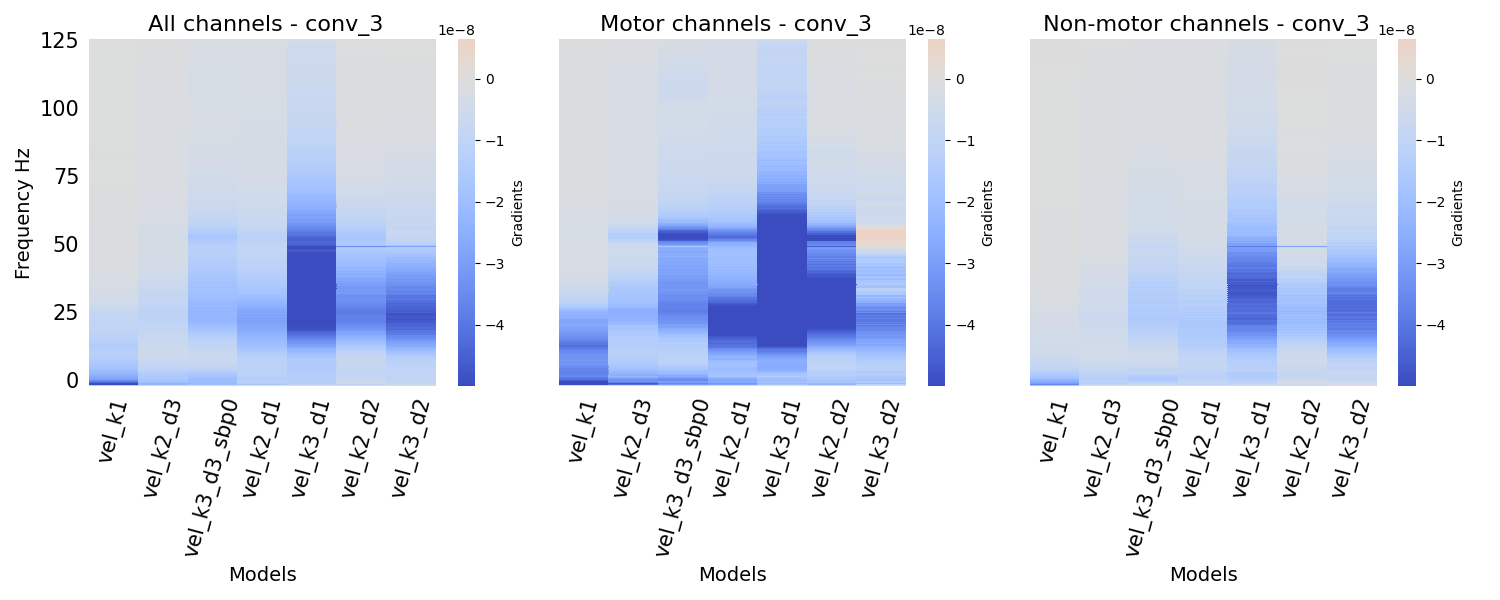
\includegraphics[width=1\linewidth]{img/ch4/vel-conv-3-layer-grads}
   \caption{}
   \label{fig:vel-conv3-layer-grads}
\end{subfigure}

\begin{subfigure}[b]{\textwidth}
   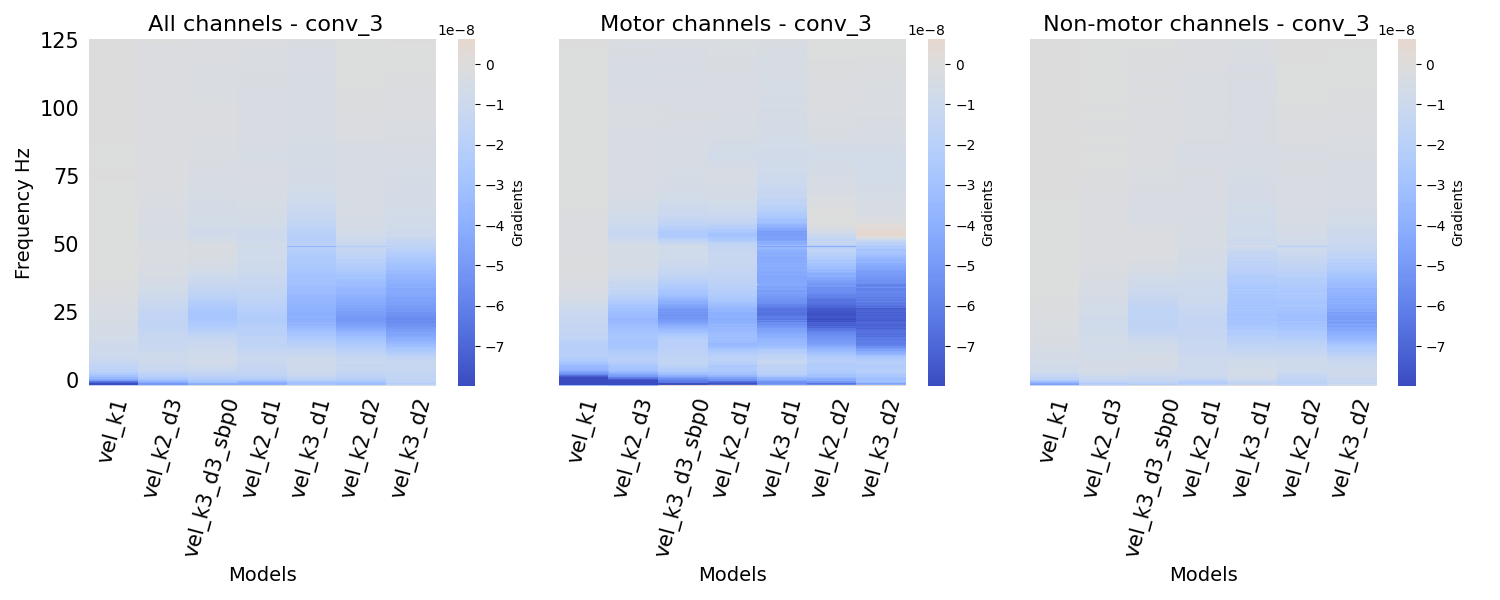
\includegraphics[width=1\linewidth]{img/ch4/vel-conv-3-layer-grads-shifted}
   \caption{}
   \label{fig:vel-conv3-layer-grads-shifted}
\end{subfigure}
\caption[Velocity: non-shifted vs. shifted gradient, full data]{Gradients of the different CNN architectures trained to decode velocity in \textbf{(a)} the original setting (causal prediction) and \textbf{(b)} in the shifted setting (acausal prediction). Full data was used for both training and validation.}
\label{fig:vel-shifted-vs-non-shifted-grads}
\end{figure}

\begin{figure}[!hpbp]
\begin{subfigure}[a]{\textwidth}
   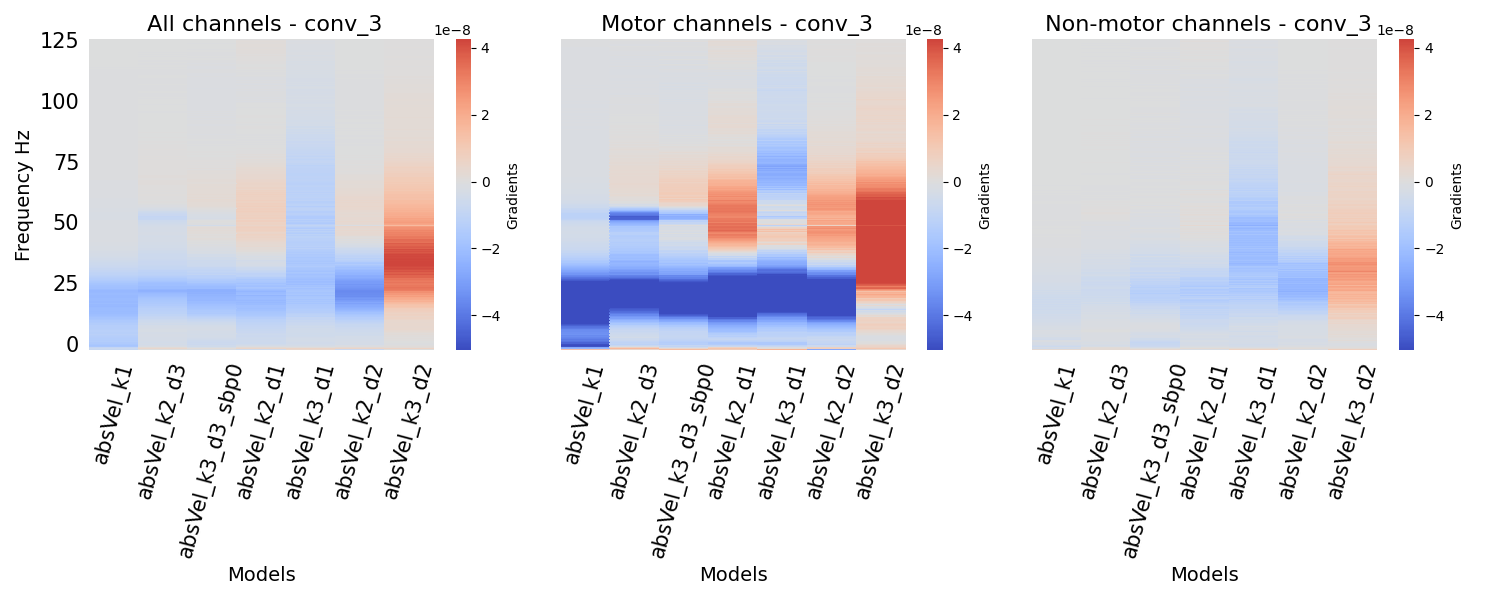
\includegraphics[width=1\linewidth]{img/ch4/absVel-conv-3-layer-grads}
   \caption{}
   \label{fig:absVel-conv-3-layer-grads}
\end{subfigure}

\begin{subfigure}[b]{\textwidth}
   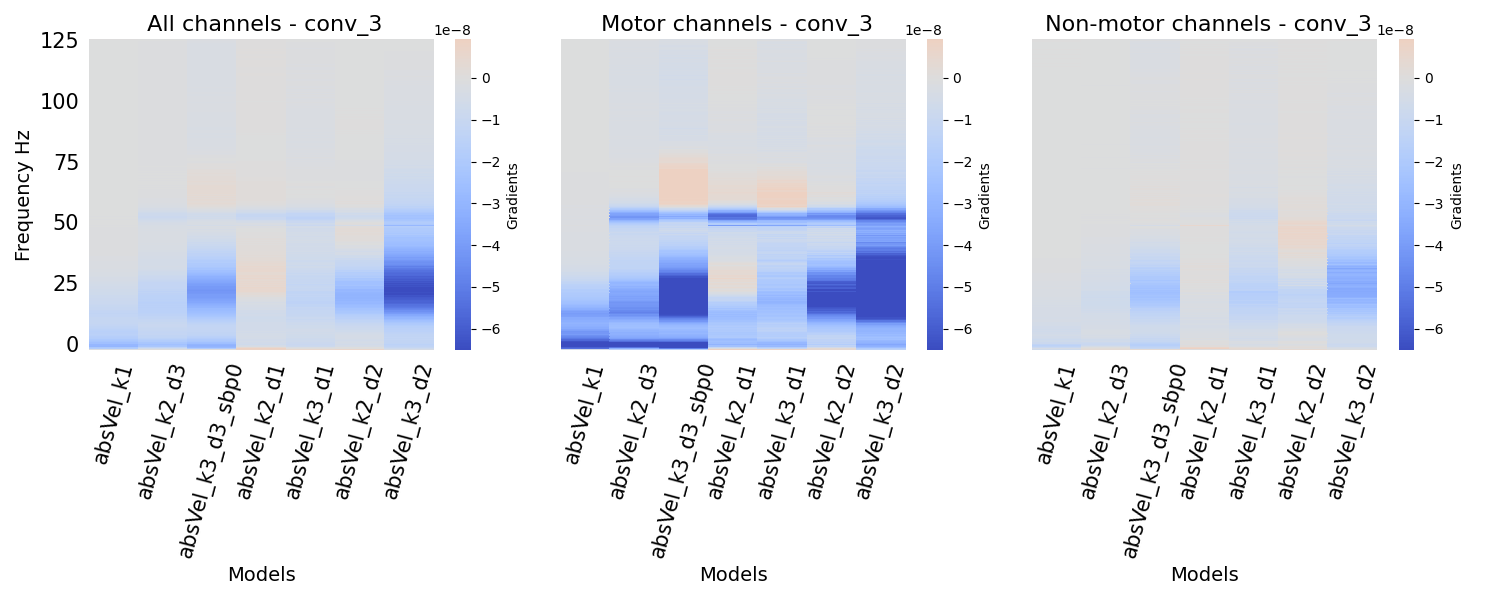
\includegraphics[width=1\linewidth]{img/ch4/absVel-conv-3-layer-grads-shifted}
   \caption{}
   \label{fig:absVel-conv-3-layer-grads-shifted}
\end{subfigure}
\caption[Absolute velocity: non-shifted vs. shifted gradients, full data]{Gradients of the different CNN architectures trained to decode absolute velocity in \textbf{(a)} the original setting (causal prediction) and \textbf{(b)} in the shifted setting (acausal prediction). Full data was used for both training and validation.}
\label{fig:absVel-shifted-vs-non-shifted-grads}
\end{figure}

% high-pass gradients with shift
\begin{figure}[!htpb]
\centering
\RawFloats
\begin{subfigure}[b]{\textwidth}
   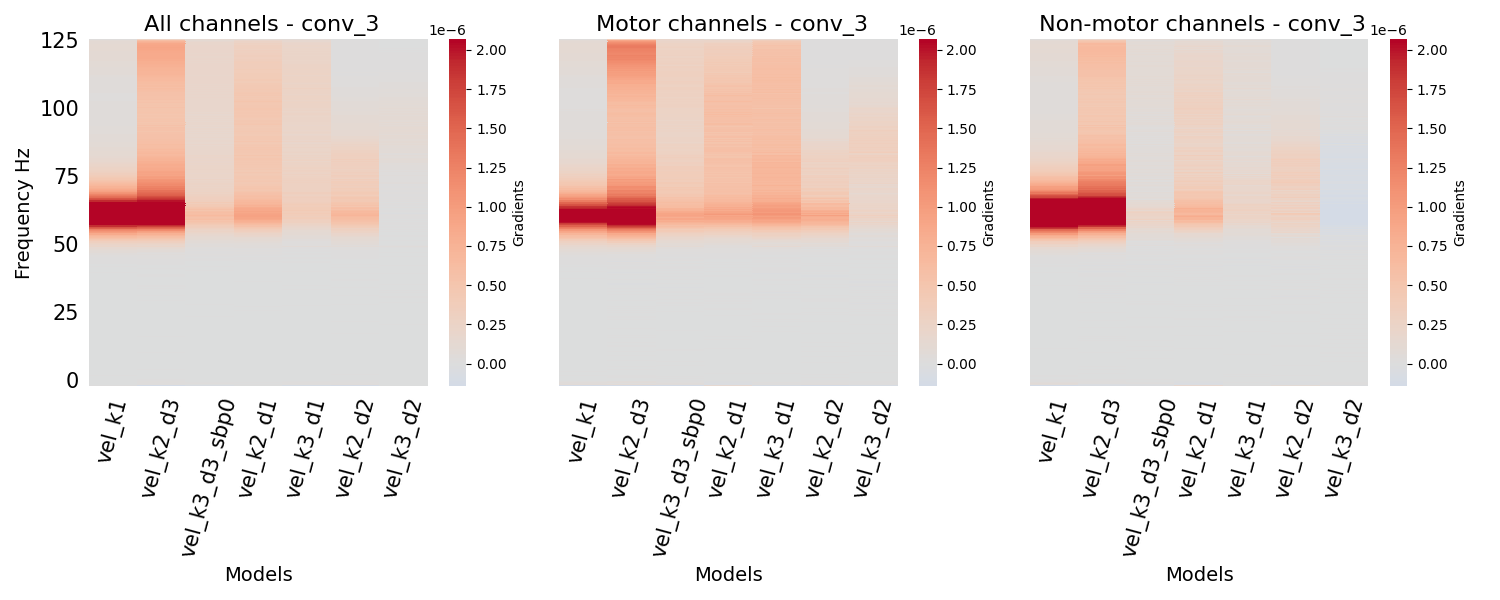
\includegraphics[width=1\linewidth]{img/ch4/vel-conv-3-layer-grads-hp}
   \caption{}
\end{subfigure}\label{fig:vel-conv3-layer-grads-hp}

\begin{subfigure}[b]{\textwidth}
   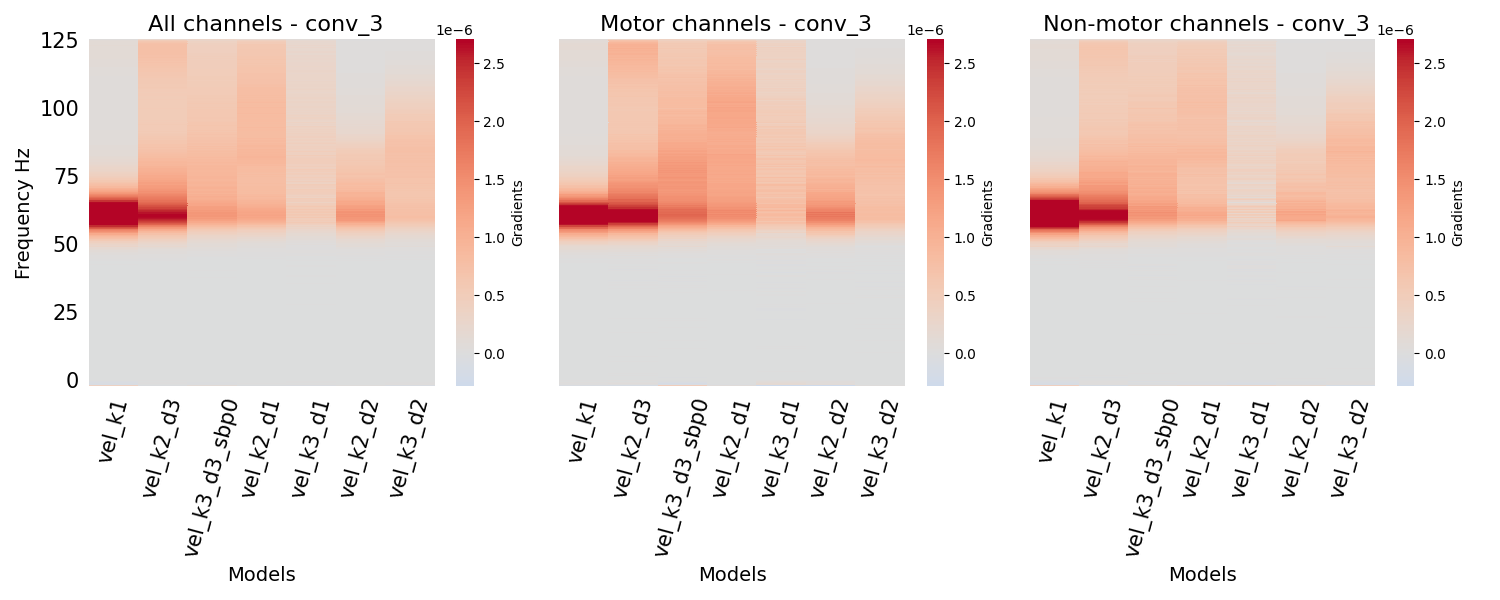
\includegraphics[width=1\linewidth]{img/ch4/vel-conv-3-layer-grads-hp-shifted}
   \caption{}
\end{subfigure}\label{fig:vel-conv3-layer-grads-shifted-hp}
\caption[Velocity: non-shifted vs. shifted gradients, high-passed data]{Gradients of the different CNN architectures trained to decode velocity in \textbf{(a)} the original setting (causal prediction) and \textbf{(b)} in the shifted setting (acausal prediction). High-passed data was used for both training and validation.}
\label{fig:vel-shifted-vs-non-shifted-grads-hp}
\end{figure}

\begin{figure}[!hpbp]
\begin{subfigure}[a]{\textwidth}
   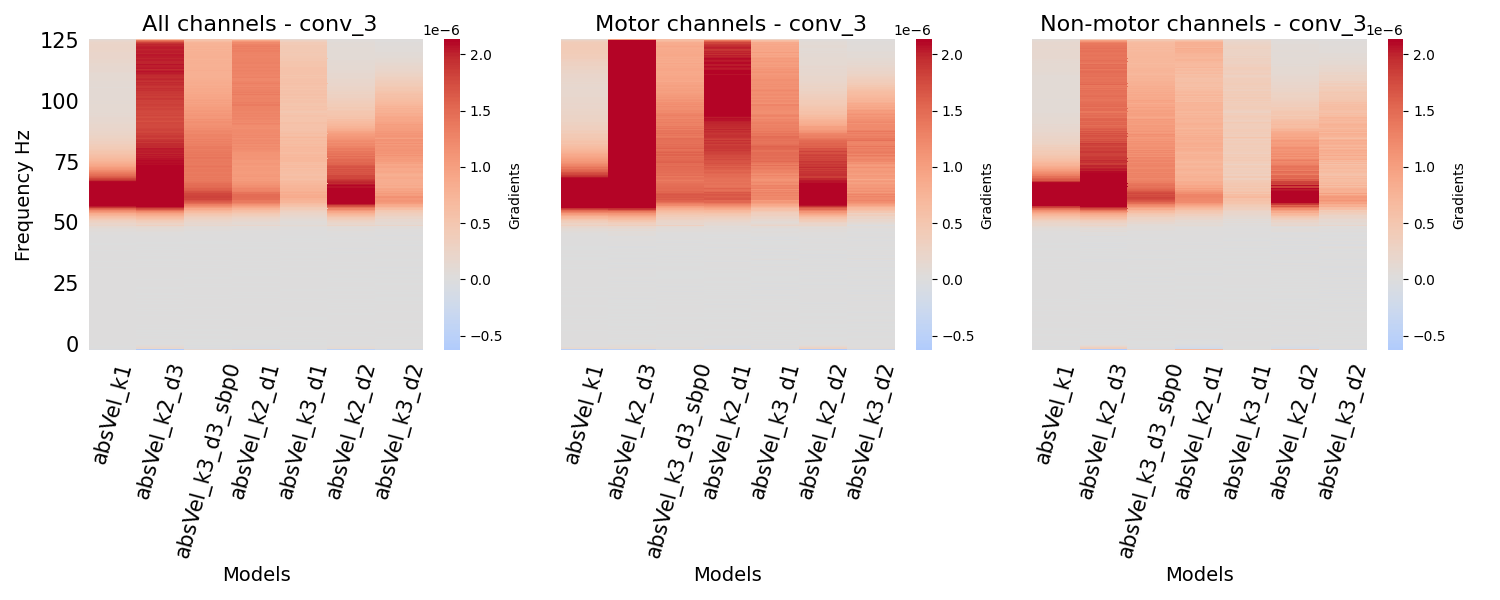
\includegraphics[width=1\linewidth]{img/ch4/absVel-conv-3-layer-grads-hp}
   \caption{}
\label{fig:absVel-conv-3-layer-grads-hp}
\end{subfigure}

\begin{subfigure}[b]{\textwidth}
   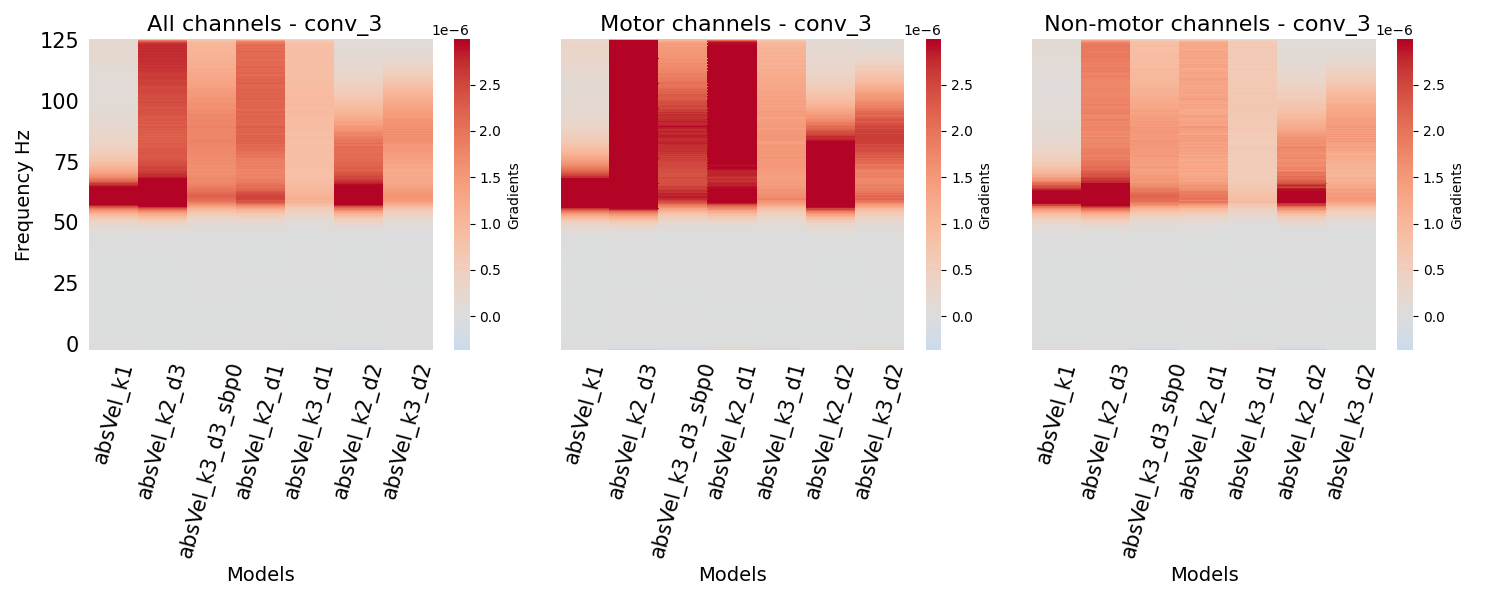
\includegraphics[width=1\linewidth]{img/ch4/absVel-conv-3-layer-grads-hp-shifted}
   \caption{}
   \label{fig:absVel-conv-3-layer-grads-shifted-hp}
\end{subfigure}
\caption[Absolute velocity: non-shifted vs. shifted gradients, high-passed data]{Gradients of the different CNN architectures trained to decode absolute velocity in \textbf{(a)} the original setting (causal prediction) and \textbf{(b)} in the shifted setting (acausal prediction). High-passed data was used for both training and validation.}
\label{fig:absVel-shifted-vs-non-shifted-grads-hp}
\end{figure}

\subsubsection{Summary}\label{subsubsec:centre-shiftig-summary}
When looking at the performances and gradients of the various CNN architectures in the shifted vs. non-shifted (original) setting, the following observation can be made.
\begin{itemize}
    \item The shift improves performance of networks 1. trained and validated on the full dataset; 2. trained on the full dataset and validated on low-passed data;
    3. trained and validated on high-passed data. This is true for both velocity and absolute velocity.
    
    \item The shift attenuates the differences in performance between the different CNNs for the full training and validation.
    When looking at graphs~\textbf{B} in both Figure~\ref{fig:shifted-performance-vel} and Figure~\ref{fig:shifted-performance-absVel}, we can see that the number of network which have a significantly better performance than the original Deep4Net (k3\_d3\_sbp0) decreases compared to \textbf{A}.
    
    \item The shift does not improve performance for the CNNs trained on full data and validated on high-pass data (graphs \textbf{G} and \textbf{H} in both~\ref{fig:shifted-performance-vel} and~\ref{fig:shifted-performance-absVel}).
    This result together with the more narrow frequency bands the networks focus on after the shift (Figures \ref{fig:vel-shifted-vs-non-shifted-grads} and \ref{fig:absVel-shifted-vs-non-shifted-grads}) show that the networks do not start focusing on high-gamma with the shift when having access to the whole frequency spectrum.
    Rather the opposite.
    They more clearly refine their focus, often on information from the lower frequency bands.
    Modulations in these low frequency bands become more informative with the shift, therefore the performance increases, and the interest of the CNNs in higher frequencies drops.
    
    \item The modulations in the high-gamma band become more informative for decoding with the shift, thus the increase in performance when training and validating on the high-passed dataset.
    Nevertheless, as we state in the point above, not even this motivates the networks to use information from the high-gamma band when having access to information from lower frequencies.
    
    \item It is true in the shifted setting, as was in the non-shifted setting, that the network without max-pool (k1) which is most solely focused on low-frequency modulations performs the best and significantly above the original Deep4Net (k3\_d3\_sbp0).
    
   
\end{itemize}

From the observations above, we can state, that the modulations in the high-gamma band are not particularly informative for velocity and absolute velocity decoding.
They contain information the CNNs are able to use for decoding. 
Nevertheless, it is not an advantage for the CNN to use high-gamma modulations when having access to all frequencies, rather it harms its performance.
It is better if the CNNs focus on low frequencies.

\subsection{Shifting the predicted time-point across receptive field}\label{subsec:shifting-the-predicted-time-point-across-receptive-field}
Besides the big shift of the predicted time-point from the edge of the receptive field to the centre, we also studied what happens if we shift the predicted time-point in small steps across the receptive field. 
The shifts range from  -1 second  to 1 second from the centre of the receptive field which we denote as 0.
When the predicted time-point is 0, we use exactly half the information from the past and half the information from the future.
When shifting towards the negative values, we use more information recorded after execution of the predicted movement (information from the future). 
Vice-versa, when shifting towards positive values, we increasingly use information recorded prior to the predicted movement coming closer to the original non-shifted setting.  
The step size is 0.1 s which is equivalent to 25 samples.
This experiments allows us to observe how the shifting gradually influences the performance and gradients of the network. 

Unlike the previous experiments we chose to perform this analysis only on one architecture, namely, the original Deep4Net (k3\_d3\_sbp0). 
The shift seems to influence the gradients of all the networks similarly.
Therefore, the amount of time and computational power necessary to train multiple networks for each of the shift steps appeared excessive.  

\subsubsection{Performance}\label{subsubsec:across-shiftig-performace}
How the performance changes with the gradual shifting of the predicted time-point is displayed in Figure~\ref{fig:shifting-performance}.
We can observe the slow decrease in performance when increasing the distance of the predicted time-point to the receptive field centre, in both directions. 
This is to be expected. 
Similarly to performance in Section~\ref{subsec:shifting-the-predicted-time-point-to-the-centre-of-the-receptive-field} we do not know if the fact that the performance peaks in the centre of the receptive field is due to having information directly preceding the movement or having access to information from the future. 
Interestingly, the decoding performance drops slower when using information predominantly from the future than when using information predominantly from the past.
To properly investigate the informativeness of past vs. future signals however, we would need to have a network with an uniform receptive field. 

\begin{figure}[!hpbp]
\centering
\begin{subfigure}[a]{\textwidth}
    \centering
   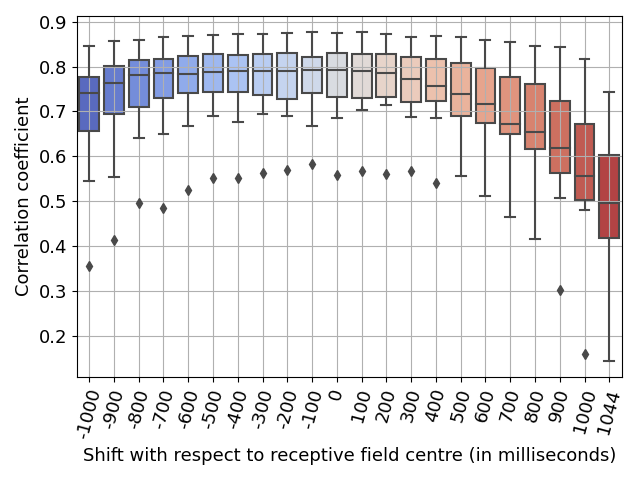
\includegraphics[width=0.7\linewidth]{img/ch4/vel-shifting-performance-comparison}
   \caption{}
   \label{fig:vel-shifting-performance}
\end{subfigure}

\begin{subfigure}[b]{\textwidth}
    \centering
   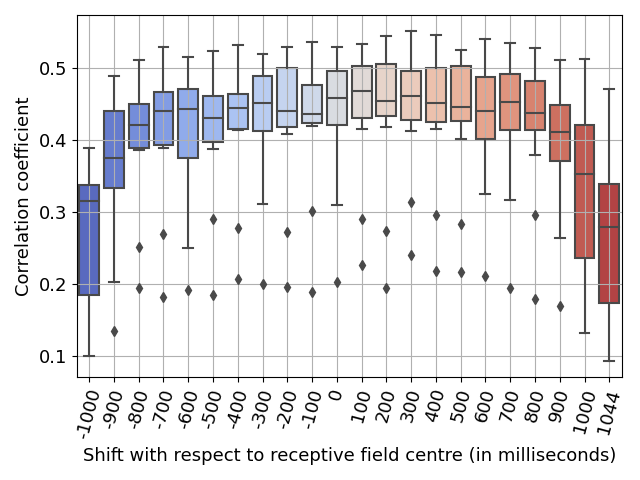
\includegraphics[width=0.7\linewidth]{img/ch4/absVel-shifting-performance-comparison}
   \caption{}
   \label{fig:absVel-shiftig-performance}
\end{subfigure}
\caption[Gradual shifting - performance]{The boxplots in \textbf{(a)} show how the CCs of the original Deep4Net (vel\_k3\_d3\_sbp0) changes for velocity decoding when shifting the predicted time-point across the receptive field.
The boxplots in \textbf{(b)} show the same but for absolute velocity. Zero miliseconds on the x-axis represent the predicted time-point being shifted to the centre of the receptive field.
Moving to the right, the network uses less information from the future and the predictions becomes more causal.
The 1041 ms mark on the x-axis is equivalent to the original fully causal prediction as described in \cite{Hammer-2021}.
When moving from 0 to the left, the network uses more and more information from the future.}
\label{fig:shifting-performance}
\end{figure}


\subsubsection{Gradients}\label{subsubsec:across-shiftig-gradients}
How the gradients are changing with the gradual shifting is visualized in Figure~\ref{fig:shifting-gradients}. 
We again chose to display one layer (the output layer) in the main text to serve as a representation of the overall trend.
The gradients of the remaining layers for both the full dataset as well as the high-passed data can be found in Appendix~\ref{appendixC}.
In the graph for absolute velocity (Figure~\ref{fig:absVel-shiftig-gradients}), we can observe the trend of broadening the frequency ranges with high gradient values when shifting the predicted time-point from the centre of the receptive field to the right towards positive values and more causal prediction which is closer to the original setting.
This is what we expected because it corresponds to the results from Section~\ref{subsec:shifting-the-predicted-time-point-to-the-centre-of-the-receptive-field} where the frequency bands with high gradient values are more narrow in the shifted setting (predicted time-point in the centre of the receptive field) and wider when performing causal prediction.
Interestingly, the frequency bands in which the network is interested broaden also when shifting the predicted time-point toward the negative values (using more information from the future). 

When plotting the same graph for velocity Figure~\ref{fig:vel-shifting-gradients}, we do not observe this behaviour so clearly.
Instead there is a periodicity in the positive and negative value of the gradients for the different values of the shift.
It is unclear why this periodicity occurs.


\begin{figure}[!htbp]
\begin{subfigure}[a]{\textwidth}
   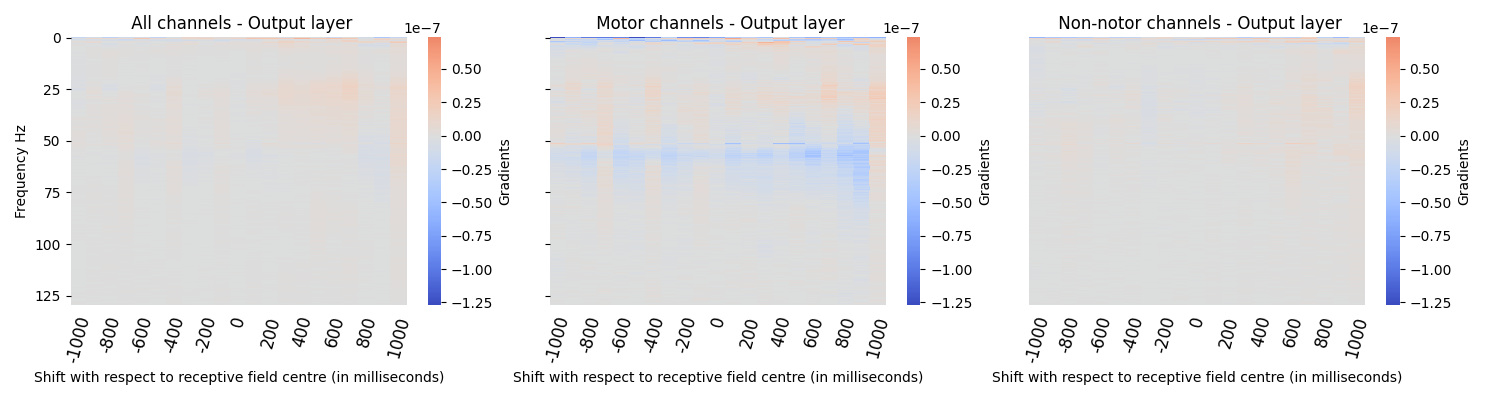
\includegraphics[width=1\linewidth]{img/appendix/C/m/vel/sbp0_m_shift_gradients_conv_classifier_all_kinds}
   \caption{}
   \label{fig:vel-shifting-gradients}
\end{subfigure}

\begin{subfigure}[b]{\textwidth}
   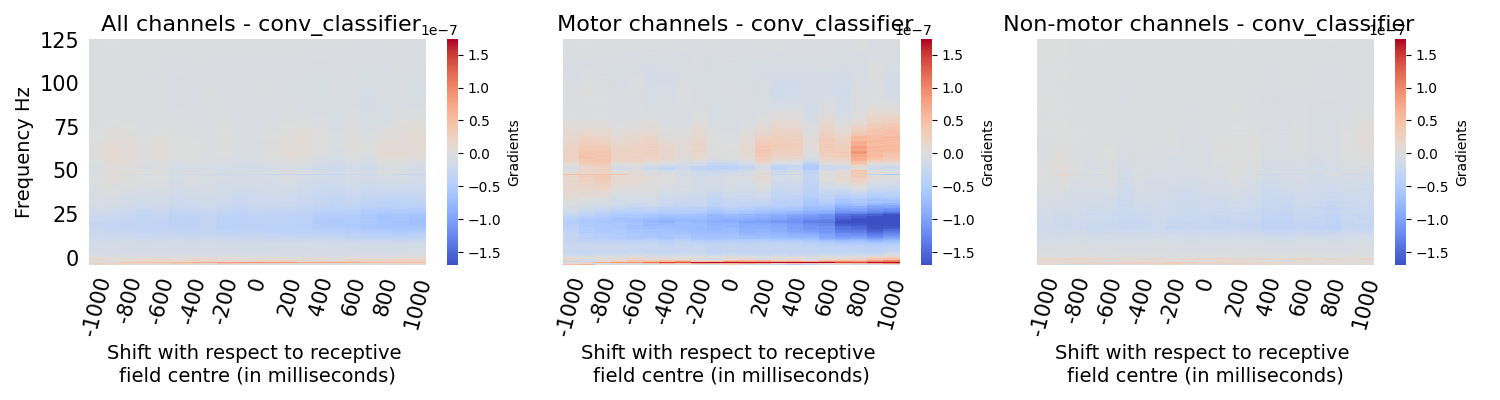
\includegraphics[width=1\linewidth]{img/appendix/C/m/absVel/sbp0_m_shift_gradients_conv_classifier_all_kinds}
   \caption{}
   \label{fig:absVel-shiftig-gradients}
\end{subfigure}
\caption[Gradual shifting - gradients]{The graph \textbf{(a)} shows the changes in gradients of the original Deep4Net (vel\_k3\_d3\_sbp0) trained to decode velocity when shifting the predicted time-point across the receptive field.
The graph \textbf{(b)} show the same but for absolute velocity. Zero miliseconds on the x-axis represent the predicted time-point being shifted to the centre of the receptive field.
Moving to the right, the network uses less information from the future and the predictions becomes more causal.
The 1041 ms mark on the x-axis is equivalent to the original fully causal prediction as described in~\cite{Hammer-2021}.
When moving from 0 to the left, the network uses more and more information from the future.}
\label{fig:shifting-gradients}
\end{figure}

\subsubsection{Summary}\label{subsubsec:across-shiftig-summary}
We have further confirmed the conclusions we drew previously in Section \ref{subsec:shifting-the-predicted-time-point-to-the-centre-of-the-receptive-field}. 
Indeed, the network seems to focus on more narrow frequency bands when given better access to information close to the predicted time-point.
This also means lower interest in the high-gamma frequency band when achieving better performance.
It corroborates what we have established so far about the information in the high-gamma band being inferior for velocity and absolute velocity decoding compared to information from lower frequency bands. 


\section{Spectral whitening}\label{sec:spectral-whitening}

How the networks react to datasets which were whitened (i. e. the amplitudes of all frequencies were normalized to 1 - see Section~\ref{subsec:modifications-to-the-dataset}) was one of our interests because when we look at the spectrum of the original signal (see Figure~\ref{fig:spectral-whitening}), the amplitudes of the frequencies decrease exponentially with increasing frequency.
This is common in biological signals and could be a reason for the CNNs to ignore high-frequencies when making predictions.
In this section we evaluate the performances and visualize gradients of all the architectures on the whitened datasets and compare the results to performances and gradients from the original non-whitened settings. 

\subsection{Performance}\label{subsec:pw-performance}

We carry out the whitening on full as well as high-passed (> 60~Hz) and low-passed datasets (< 40~Hz) and their combinations. 
Figure~\ref{fig:pw-performance} shows how the predictions change compared to predictions on non-whitened signals.
We summarize the behavior the different datasets in the points below:
\begin{itemize}
    \item \textbf{Full training and validation:} It is obvious that for the full training and validation for both velocity (Figure~\ref{fig:vel-pw-performance} graphs~\textbf{A}~and~\textbf{B}) and absolute velocity (Figure~\ref{fig:absVel-pw-performance} graphs~\textbf{A}~and~\textbf{B}), the correlation coefficient of all networks dropped significantly. The network experiencing the lowest drop of performance due to spectral whitening was the network without max-pool (\{variable\}\_k1).

    \item \textbf{Full training and low-pass validation:} The drop of performance between full training and validation and full training and low-pass validation, was bigger with whitening (graphs \textbf{C} and \textbf{D} in Figures~\ref{fig:vel-pw-performance} and \ref{fig:absVel-pw-performance}) compared to the original non-shifted setting. This suggests that spectral whitening increased the use of the high-gamma frequency when having access to all frequencies.  
    
    \item \textbf{High-pass training and validation:} When looking at graphs \textbf{E} and \textbf{F} in both Figure~\ref{fig:vel-pw-performance} and Figure~\ref{fig:absVel-pw-performance} we see that in the case of the high-passed datasets the performance did not increase or decrease significantly for any of the networks. 
    This shows that the low amplitudes of these frequencies are not the issue when decoding from them because increasing it does not aid the network in making predictions from them. Neither does increasing it harm them.
    
    \item \textbf{Full training and high-pass validation:} (graphs~\textbf{G} and \textbf{H} in Figure~\ref{fig:vel-pw-performance} and Figure~\ref{fig:absVel-pw-performance})
    was the only scenario where spectral whitening helped the CNNs to achieve better CCs. 
    In the case of velocity \ref{fig:vel-pw-performance} a statistically significant increase compared to the same non-whitened setting was only for the vel\_k1 network.
    In the case of absolute velocity \ref{fig:absVel-pw-performance} five out of the seven architectures experienced a statistically significant increase in performance due to spectral whitening.
    The CCs increases after spectral whitening in this last scenario show that at least some of networks indeed learned to use more high-gamma when having access to full data.
\end{itemize}


\begin{figure}[!htbp]
\begin{subfigure}[a]{\textwidth}
   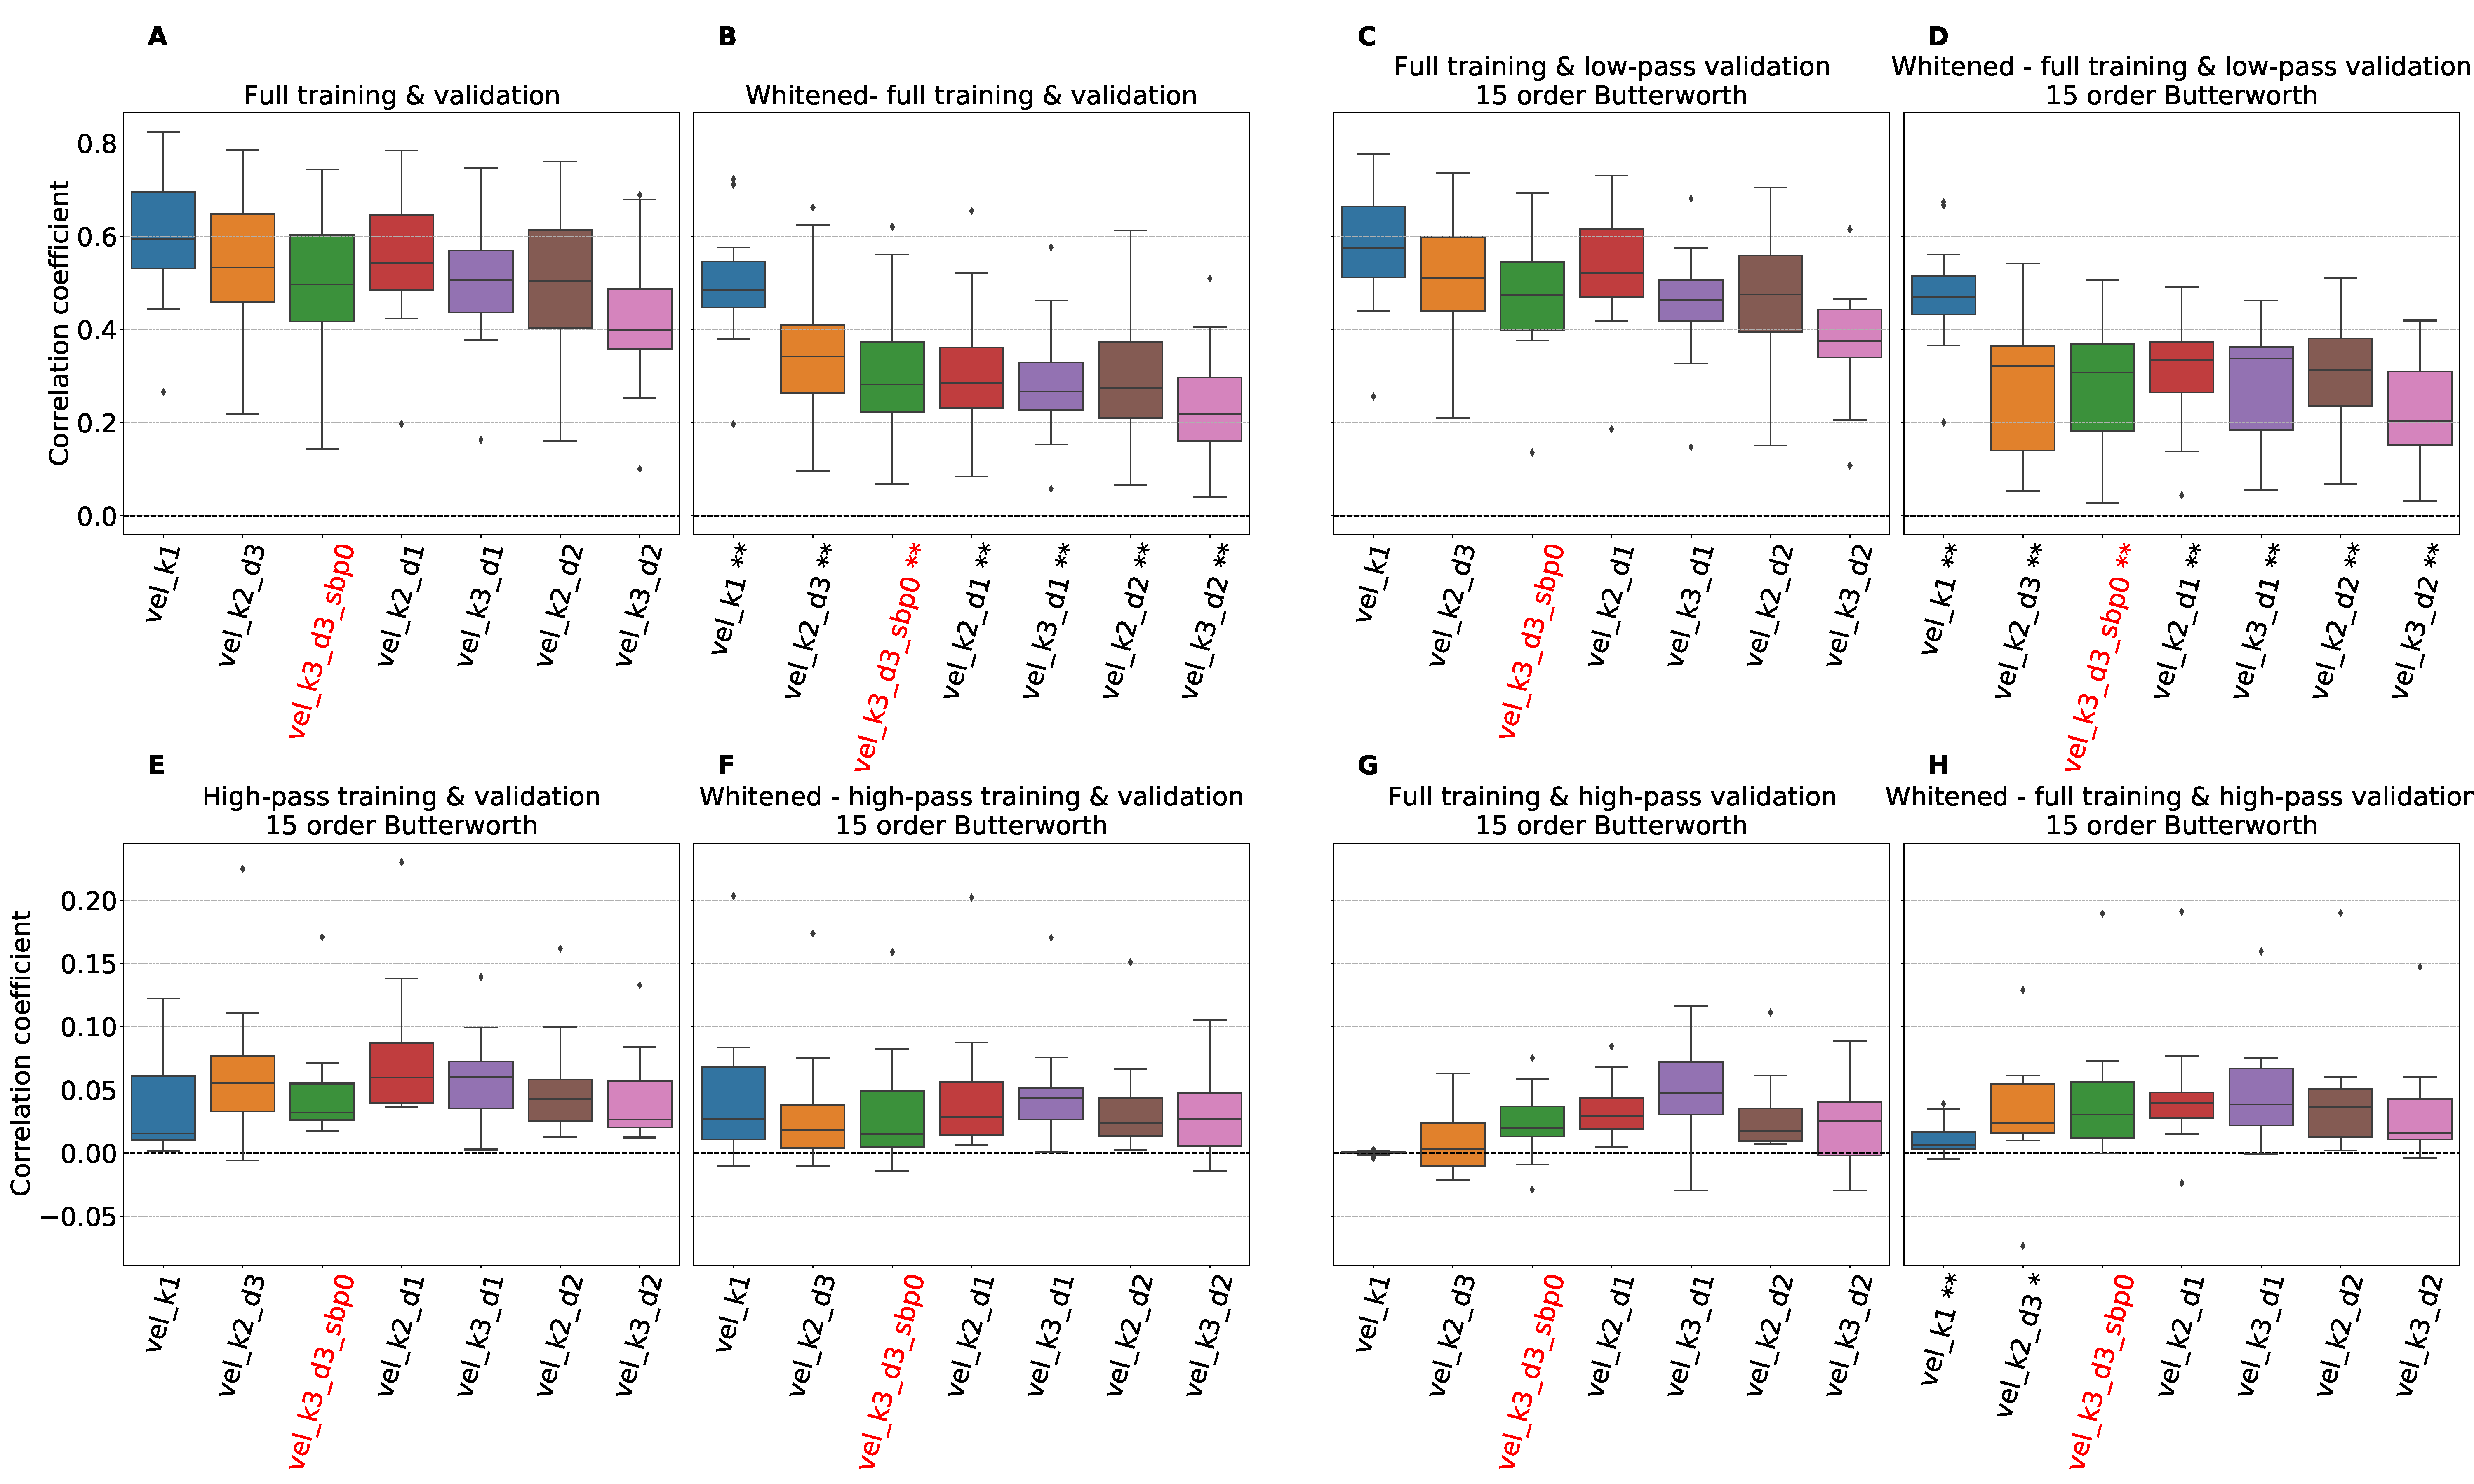
\includegraphics[width=1\linewidth]{img/ch4/vel-pw-vs-non-pw-performance}
   \caption{\textbf{Velocity} decoding correlation coefficients comparison between the networks trained on non-whitened datasets \textbf{Graphs A, C, E, G} and the whitened dataset \textbf{Graphs B, D, F, H}.
   In all settings \textbf{A - E} the Deep4Net (k3\_d3\_sbp0) from~\cite{Hammer-2021} is labeled red.
   \\ \textbf{Graphs A} and \textbf{B} compare the performance of the networks when trained and validated on the full dataset.
   The stars in \textbf{B} denote CCs significantly lower compared to CCs of the same architecture in \textbf{A} (** p <0.01), (* p < 0.05), Wilcoxon signed rank test.
   \\\textbf{Graphs C} and \textbf{D} show the correlation coefficients of the networks trained on full data and validated on low-passed data.
   The stars in \textbf{D} denote if the CCs are significantly lower compared to CCs of the same architecture in \textbf{C} (** p <0.01), (* p < 0.05), Wilcoxon signed rank test.
   \\\textbf{Graphs E} and \textbf{F} compare the CCs of the CNNs when trained and validated on high-passed data.
   The stars in \textbf{F} denote CCs significantly lower compared to CCs of the same architecture in \textbf{E} (** p <0.01), (* p < 0.05), Wilcoxon signed rank test.
   \textbf{Graphs G} and \textbf{H} compare performance when trained on full data and validated on high-passed data.
   The stars in \textbf{H} denote CCs significantly lower compared to CCs of the same architecture in \textbf{G} (** p <0.01), (* p < 0.05), Wilcoxon signed rank test.}
   \label{fig:vel-pw-performance}
\end{subfigure}
\end{figure}
\clearpage   

\begin{figure}[!htbp]\ContinuedFloat
\begin{subfigure}[b]{\textwidth}
   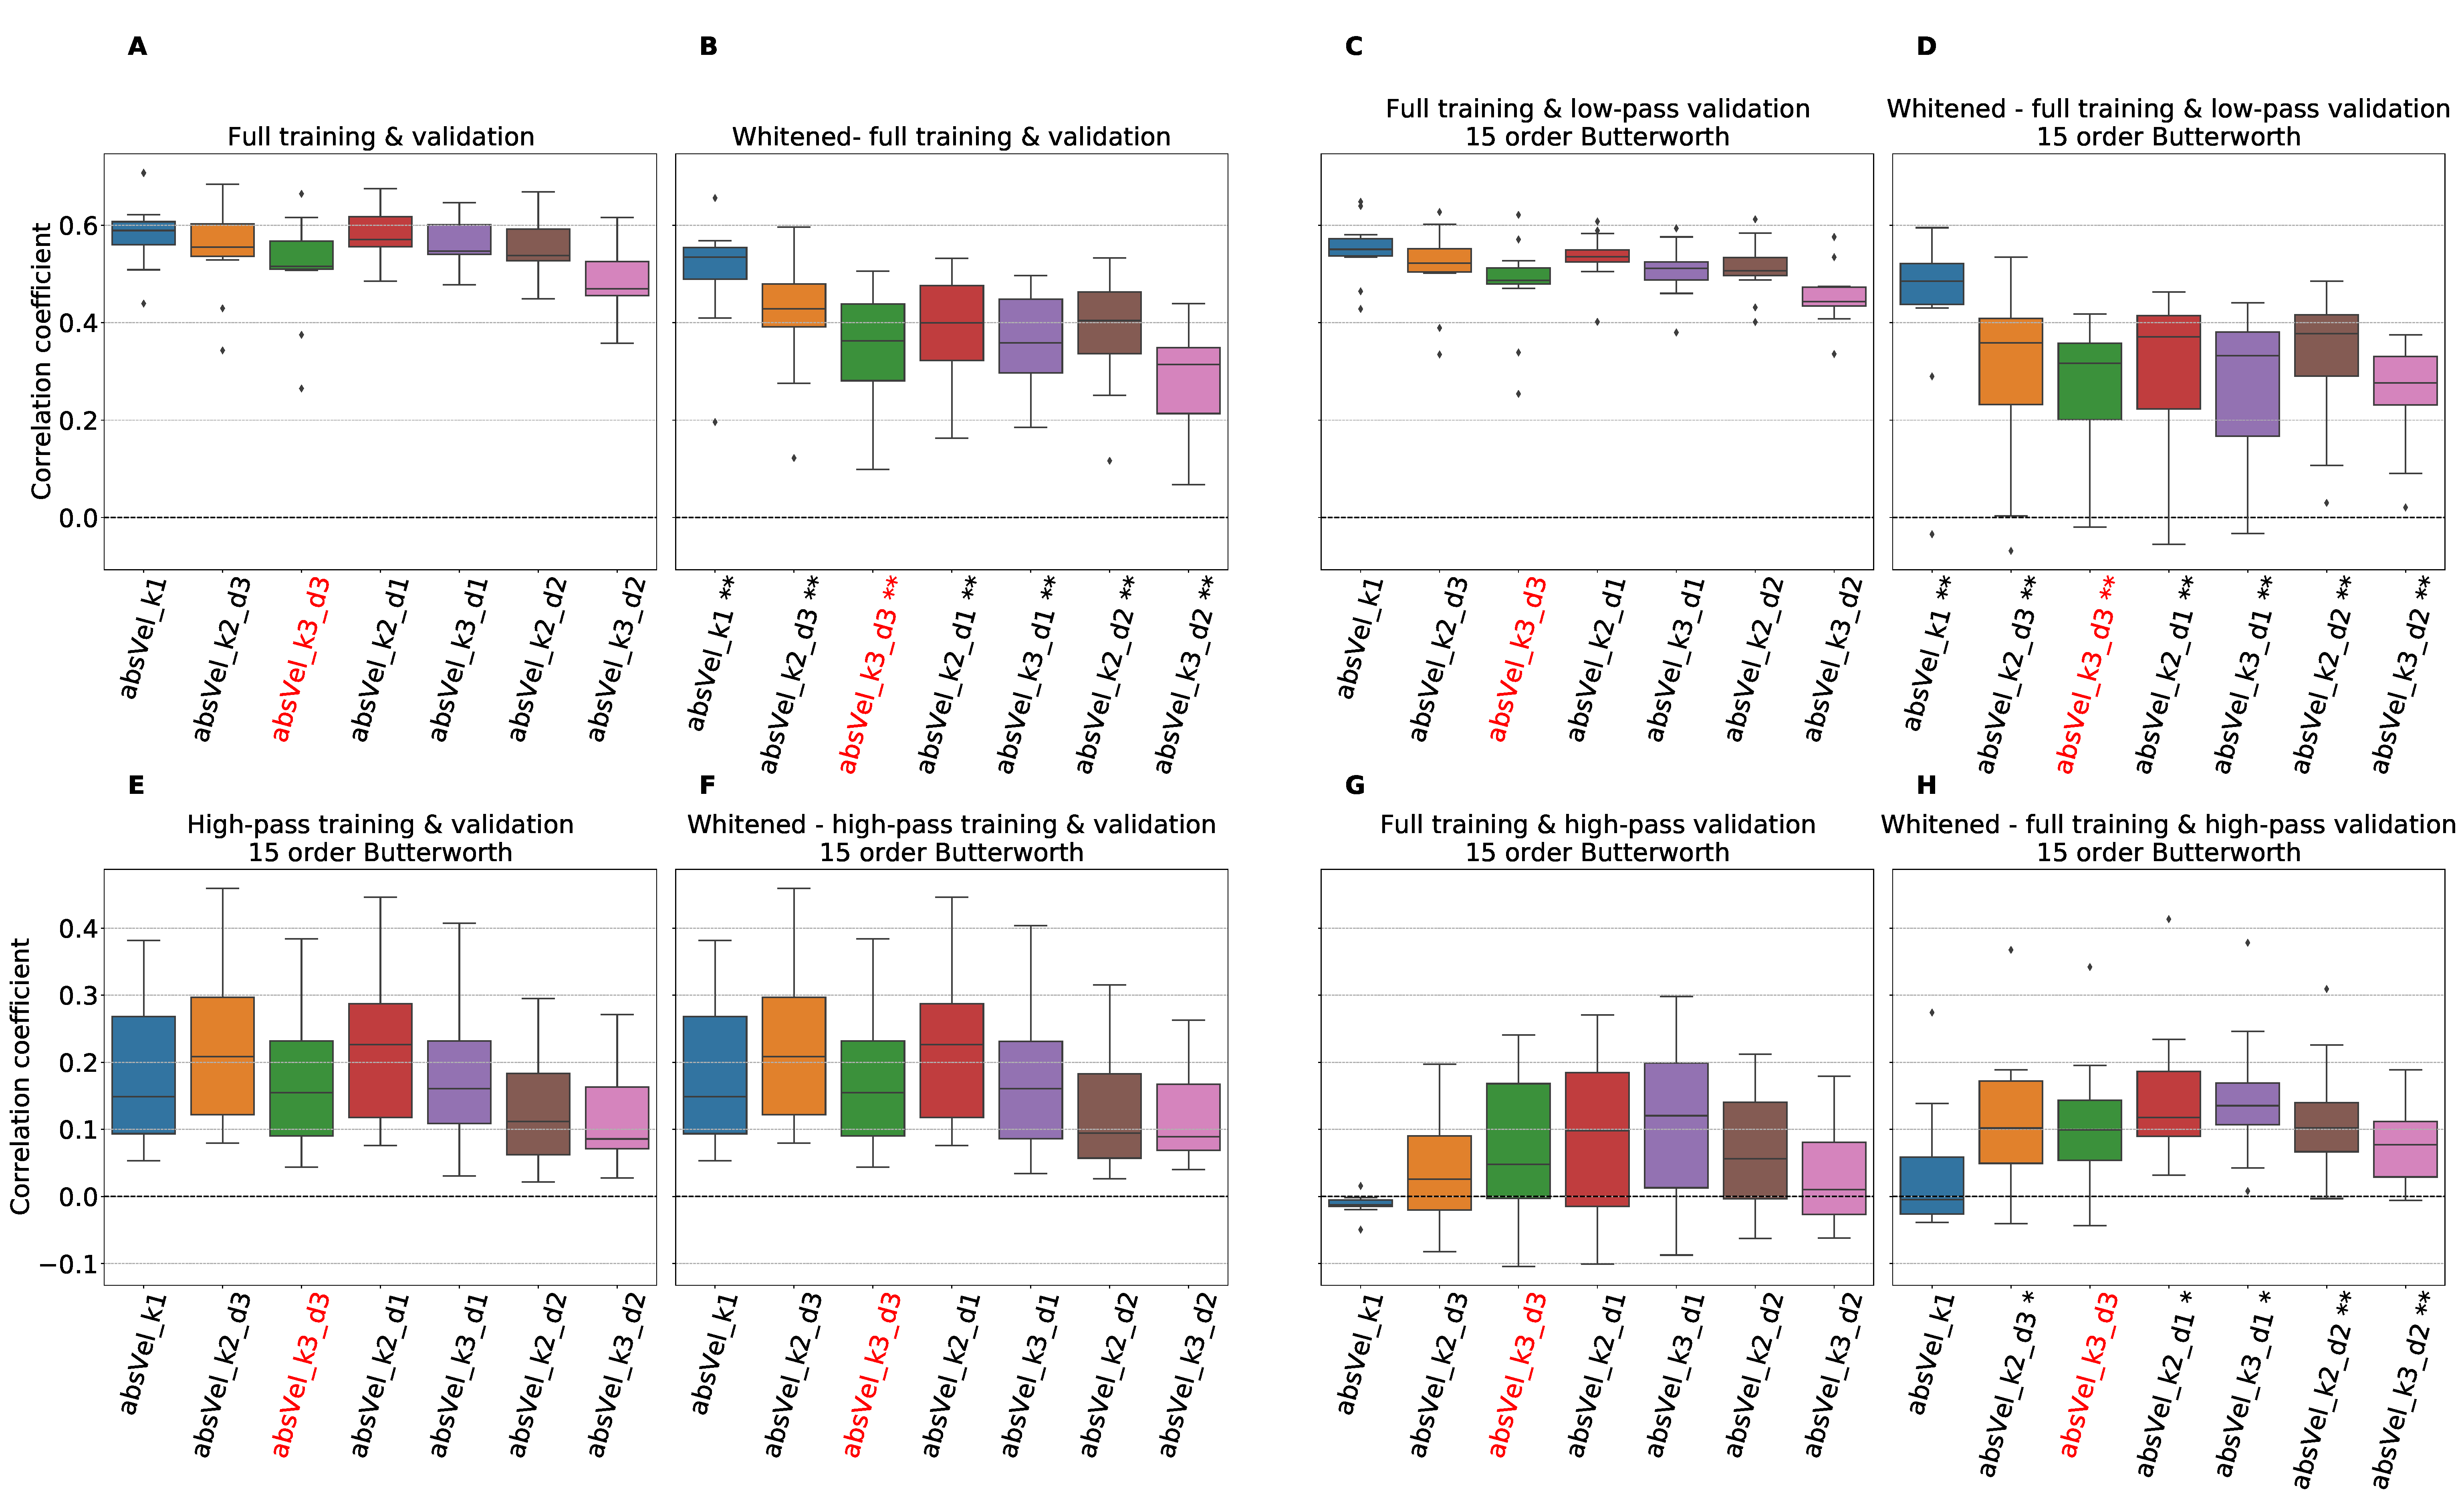
\includegraphics[width=1\linewidth]{img/ch4/absVel-pw-vs-non-pw-performance}
   \caption{\textbf{Absolute velocity} decoding correlation coefficients comparison between the networks trained on the non-whitened datasets \textbf{Graphs A, C, E, G} and the whitened dataset \textbf{Graphs B, D, F, H}.
   In all settings \textbf{A - E} the Deep4Net (k3\_d3\_sbp0) from~\cite{Hammer-2021} is labeled red.
   \\ \textbf{Graphs A} and \textbf{B} compare the performance of the networks when trained and validated on the full dataset.
   The stars in \textbf{B} denote CCs significantly lower compared to CCs of the same architecture in \textbf{A}. (** p <0.01), (* p < 0.05), Wilcoxon signed rank test.
   \\\textbf{Graphs C} and \textbf{D} show the correlation coefficients of the networks trained on full data and validated on low-passed data.
   The stars in \textbf{D} denote if the CCs are significantly lower compared to CCs of the same architecture in \textbf{C} (** p <0.01), (* p < 0.05), Wilcoxon signed rank test.
   \\\textbf{Graphs E} and \textbf{F} compare the CCs of the CNNs when trained and validated on high-passed data.
   The stars in \textbf{F} denote CCs significantly lower compared to CCs of the same architecture in \textbf{E}. (** p <0.01), (* p < 0.05), Wilcoxon signed rank test.
   \textbf{Graphs G} and \textbf{H} compare performance when trained on full data and validated on high-passed data.
   The stars in \textbf{H} denote CCs significantly lower compared to CCs of the same architecture in \textbf{G}. (** p <0.01), (* p < 0.05), Wilcoxon signed rank test.}
   \label{fig:absVel-pw-performance}
\end{subfigure}
\caption[Spectral whitening - performance comparison]{}
\label{fig:pw-performance}
\end{figure}

\subsection{Gradients}\label{subsec:pw-gradients2}
When looking at the gradients of the networks trained on whitened data in Figure~\ref{fig:pw-last-layer-grads}\footnote{We present the gradients only for the output layer to highlight our observations. 
The results for all layers can be found in Appendix~\ref{appendixD}.}, we observe that the networks indeed use modulations in the high-gamma frequency bands for their predictions. 
This finding is also supported by the fact that the networks trained on full data and validated on high-passed data experienced an increase in the correlations coefficients with spectral whitening.
For absolute velocity, the gradients have high values in bands across the whole frequency range. Interestingly, for velocity, instead of having more uniform gradients across all frequencies, they partially invert their focus from low frequencies to high-frequencies.

Among CNNs decoding velocity, the only architecture which stays mostly focused on frequencies below 25~Hz is the vel\_k1 CNN which is the network without max-pool layers.
The same is true for absolute velocity, where the network without max-pools (absVel\_k1) also stays mostly focused on the low frequencies even though a slight increase in gradient values for frequencies around 75~Hz can be observed. 
We can combine this information about the gradients with the performance graphs in Figure~\ref{fig:pw-last-layer-grads}, where we can see, that the networks without max-pools which were least influenced by the spectral whitening in terms of focusing on higher frequencies are those for which the CCs dropped least.
This fact suggests that using information from the high-gamma frequency is possible, but it does not seem to help achieve better correlation coefficients. 
On the contrary, using information from the high-gamma frequency band is not helpful for better network performance and using information in the low frequencies leads to better prediction power even on the whitened datasets.

\begin{figure}[!htbp]
\begin{subfigure}[a]{\textwidth}
   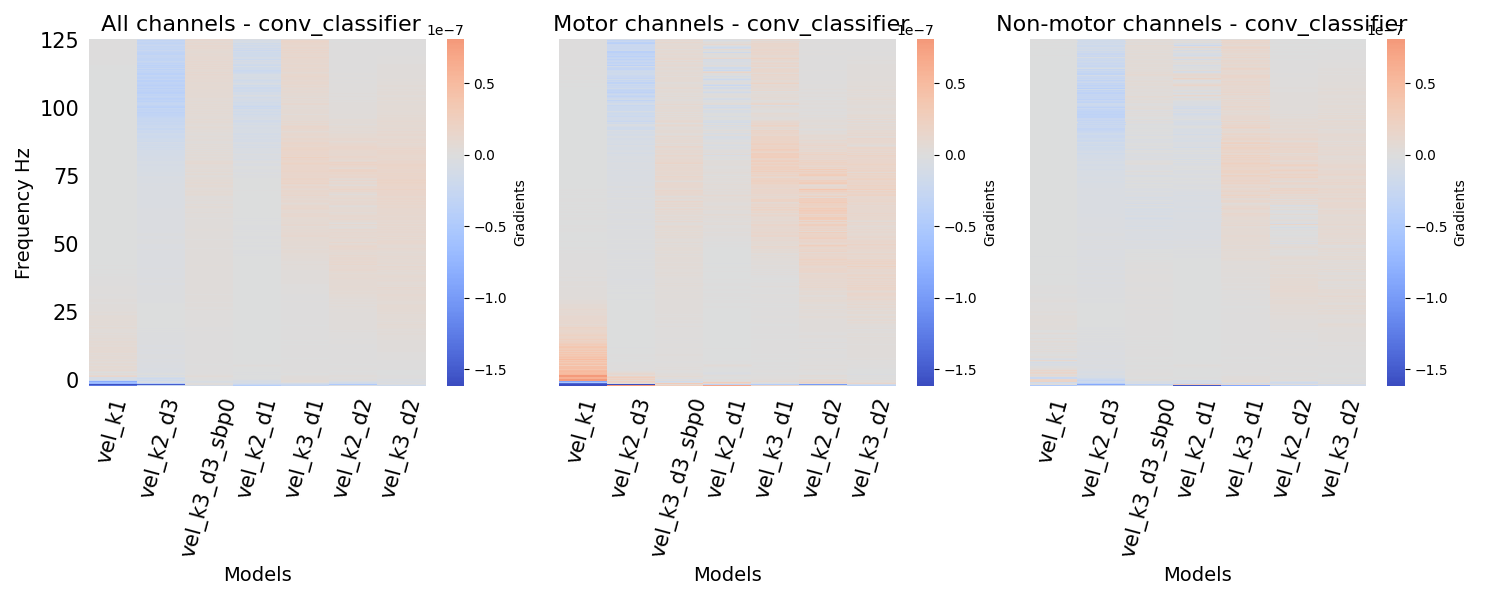
\includegraphics[width=1\linewidth]{img/ch4/vel-pw-last-layer-grads}
   \caption{}
   \label{fig:vel-pw-last-layer-grads}
\end{subfigure}

\begin{subfigure}[b]{\textwidth}
   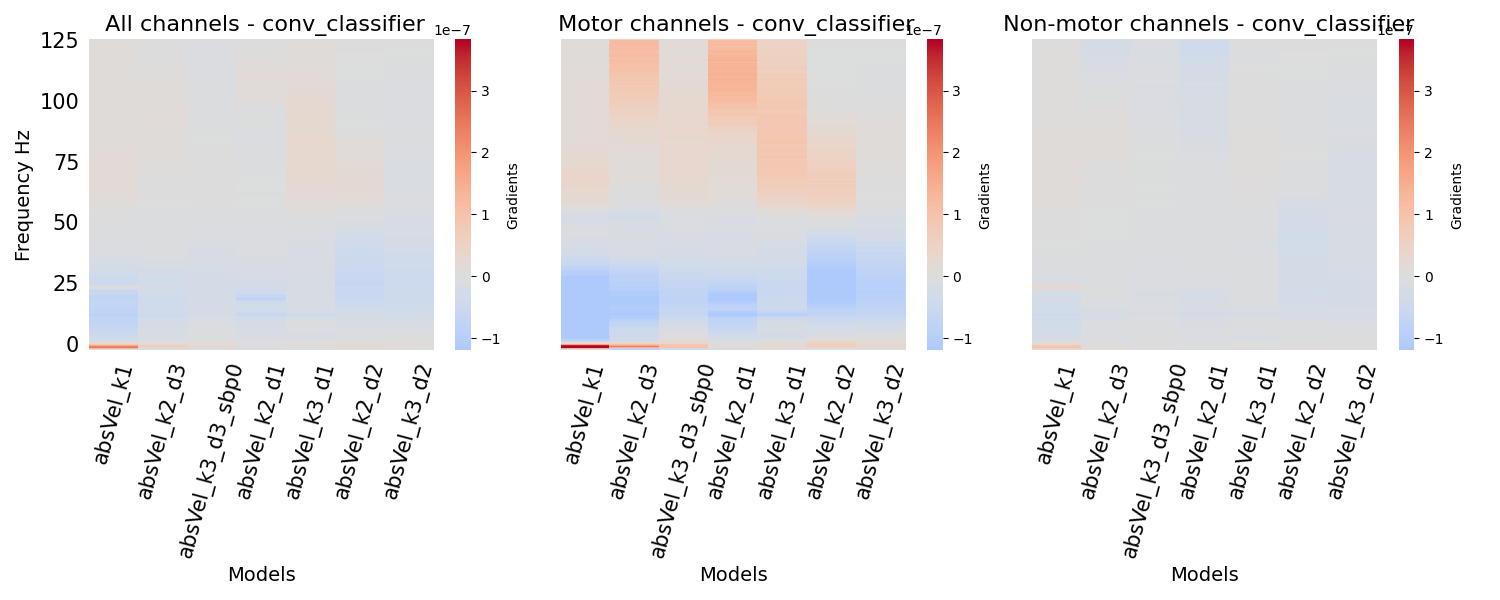
\includegraphics[width=1\linewidth]{img/ch4/absVel-pw-last-layer-grads}
   \caption{}
   \label{fig:absVel-pw-last-layet-grads}
\end{subfigure}
\caption[Spectral whitening - gradients]{Gradients of networks trained to decode \textbf{(a)} velocity and \textbf{(b)} absolute velocity on spectrally-whitened datasets}
\label{fig:pw-last-layer-grads}
\end{figure}

Overall spectral whitening forced most of the networks into using high-gamma. 
At the same time, it harmed the prediction power of the networks.
We can therefore again state, that while information in the high-gamma frequency band holds information about velocity and especially absolute velocity, the networks perform better when they focus on information from lower frequency bands. 
And removing the max-pool layer helps the networks to utilize information in the low frequency bands more effectively even on the whitened dataset.


